% -*- coding: utf-8; -*-

\chapter{Geração Semiautomática}
\label{ch:gordon}

	\textit{Kindlmann e Durkin}~\cite{gordon} foram uns dos primeiros a gerar funções de transferência para visualizar as fronteiras de um volume de dados. Apesar de ter sido publicado há quase 20 anos e de possuir alguns pontos fracos já estudados por outros, seu trabalho ainda é o mais equilibrado no quesito \quote{Geração automática \textit{X} Controle do usuário}. Isso deve-se ao fato de que seu método gera bons resultados com funções de transferência 1D, que são naturalmente mais intuitivas ao usuário. Além disso, exige intervenção mínima do usuário para gerar a FT, ao mesmo tempo que permite um controle fino sobre como a fronteira deve ser apresentada visualmente. Por esse motivo, este trabalho foi escolhido como base para pesquisa e desenvolvimento desta dissertação e será apresentado neste capítulo em 3 seções. A Seção~\ref{sec:gordon.bound} define o conceito de fronteira e explica como identificá-las. A obtenção do modelo matemático que gera a função de transferência 1D e 2D pode ser encontrada na Seção~\ref{sec:gordon.ft}, bem como seus respectivos resultados. Por fim, o método é avaliado na Seção~\ref{sec:gordon.aval}.
	
\section{Detecção de Fronteiras}
\label{sec:gordon.bound}

\begin{figure}[b]
	\centering
	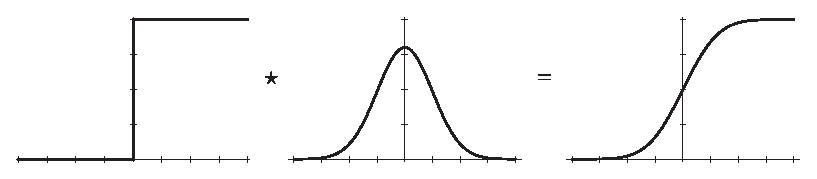
\includegraphics[width=1\textwidth]{images/g_boundary_model}
	\caption{Comportamento das funções degrau, gaussiana e erro, respectivamente~\cite{gordon}.}
	\label{fig:boundary_model}
\end{figure}

	Kindlmann e Durkin partem da premissa de que todos os materiais representados no volume de dados possuem propriedades físicas homogêneas. Dessa forma, toda fronteira seria caracterizada por uma variação abrupta na intensidade lida do volume e poderia ser representada pela função degrau. No entanto, devido aos dispositivos responsáveis pela aquisição de dados, as fronteiras são comumente borradas com uma resposta gaussiana na frequência. Por esse motivo, o comportamento de uma fronteira em um volume de dados é melhor representado pela convolução da função degrau com uma gaussiana. O resultado dessa convolução é a função \textit{erf(x)}, ou função \textit{erro}, ilustrada na Figura~\ref{fig:boundary_model}.

	\textit{erf(x)} é uma função contínua cuja imagem varia de $-1$ a $1$. Como uma fronteira pode variar entre quaisquer dois valores escalares contidos no volume, \textit{erf(x)} deve ser escalada para variar de $v_{min}$ a $v_{max}$. Assim, a função $f(x)$ que modela uma fronteira é definida pela equação~\eqref{eq:boundary}. O esticamento da função $ f(x) $ em relação à $ erf(x) $ pelo fator $ \sigma\sqrt{2} $ será explicado mais à frente.
	\\

\begin{equation} \label{eq:boundary}
	v = f(x) = v_{min} + (v_{max} - v_{min}) \frac{1 + erf(\frac{x}{\sigma\sqrt{2}})}{2}
\end{equation} \

	Uma outra maneira de interpretar a fronteira é como sendo uma das isosuperfícies entre $v_{min}$ e $v_{max}$. Uma vez que a derivada direcional indica a taxa de variação de uma função em uma determinada direção, a isosuperfície que melhor representa a fronteira é aquela que possui a maior derivada, pois esta estará localizada no ponto da fronteira em que a variação entre $v_{min}$ e $v_{max}$ for maior.
	
\begin{figure}[h]
	\centering
	%	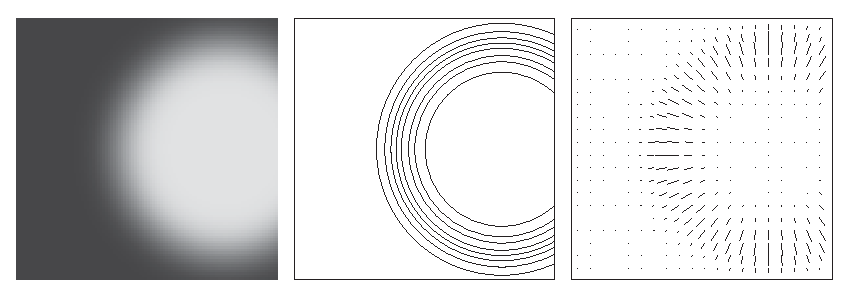
\includegraphics[width=1\textwidth]{images/grad}
	\subfigure[Intensidades]{
		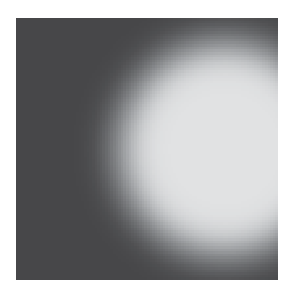
\includegraphics[width=0.3\textwidth]{images/g_cilynder}
		\label{fig:g_isosurfaces_a}
	}
	\subfigure[Isosuperfícies]{
		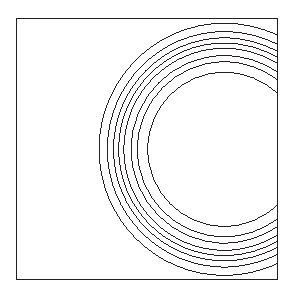
\includegraphics[width=0.3\textwidth]{images/g_isosurfaces}
		\label{fig:g_isosurfaces_b}
	}
	\subfigure[Vetores gradiente]{
		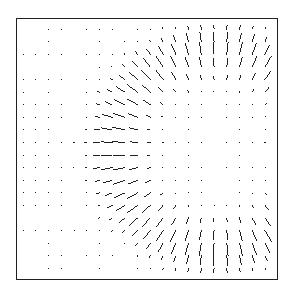
\includegraphics[width=0.3\textwidth]{images/g_grads}
		\label{fig:g_isosurfaces_c}
	}
	\caption{Visão em corte de um cilindro~\cite{gordon}.}
	\label{fig:g_isosurfaces}
\end{figure}
	
	No entanto a derivada não pode ser calculada em qualquer direção. Para que a derivada indique a variação entre $v_{min}$ e $v_{max}$ a direção deve ser aquela que parte de um voxel com valor $v_{min}$ para um com valor $v_{max}$, atravessando os valores intermediários. Essa direção desejada seria então a normal das isosuperfícies, uma vez que esta é sempre perpendicular ao plano que tangencia a isosuperfície e, portanto, sempre aponta na direção de outra isosuperfície. Nesse caso, o vetor normal pode ser aproximado pelo vetor gradiente, uma vez que este aponta na direção que possui a maior variação de valores do volume e, portanto, também na direção da próxima isosuperfície.
	
	%%% Seguindo a premissa de que a fronteira é uma variação rápida de alta intensidade, ela é melhor representada pela isosuperfície que apresenta a maior derivada. Como o vetor gradiente aponta na direção da maior taxa de variação de uma função, ele pode ser usado para caminhar entre as isosuperfícies de um volume. Assim, através da avaliação da derivada na direção do gradiente, a isosuperfície que representa corretamente a fronteira pode ser obtida.

	A Figura~\ref{fig:g_isosurfaces}~\ref{fig:g_isosurfaces_a} mostra o corte de um volume cilíndrico, onde $v_{min}$ foi mapeado para cinza escuro e $v_{max}$ para cinza claro. As isosuperfícies existentes entre esses valores estão ilustradas na Figura~\ref{fig:g_isosurfaces}~\ref{fig:g_isosurfaces_b}, enquanto a Figura~\ref{fig:g_isosurfaces}~\ref{fig:g_isosurfaces_c} exibe os vetores gradiente do volume. Percebe-se que os gradientes se aproximam das normais das isosuperfícies, apontando sempre para uma próxima isosuperfície, como discutido anteriormente.
		
\begin{figure}[h]
	\centering
	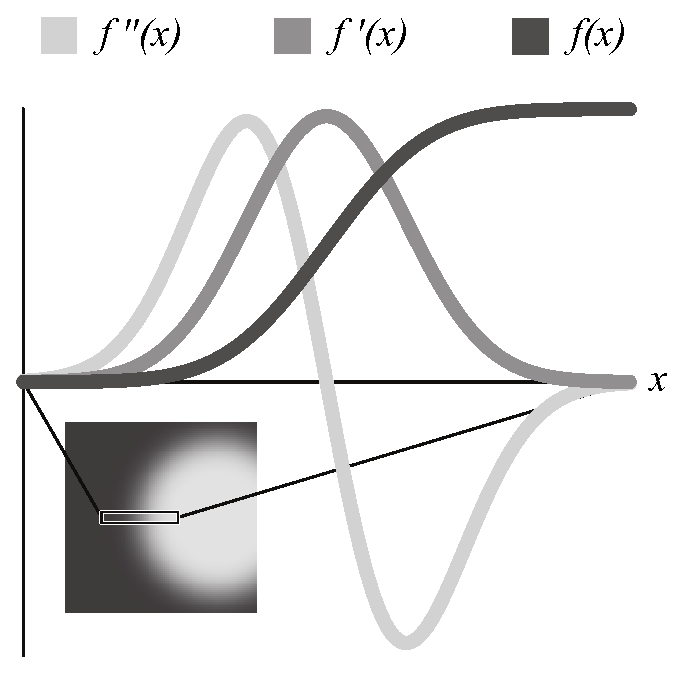
\includegraphics[width=0.5\textwidth]{images/g_functions_all}
	\caption{Comportamento de $f(x)$, $f'(x)$ e $f''(x)$ na direção do gradiente, em função da posição no volume~\cite{gordon}.}
	\label{fig:g_functions}
\end{figure}
	
	A Figura~\ref{fig:g_functions} mostra o comportamento da primeira e segunda derivadas na presença de uma fronteira. Como esperado, o ponto de maior primeira derivada e, portanto, segunda derivada igual a zero, identificam a posição exata da fronteira. Como a curva $f'(x)$ se comporta como uma distribuição normal, o termo $ \sigma\sqrt{2} $ foi adicionado a $ f(x) $ para que ao derivá-la $ f'(x) $ seja de fato uma função gaussiana com desvio padrão $ \sigma $.
	
	No entanto, as curvas apresentadas apenas possuem essa forma na direção do gradiente. Isso dificulta expressar graficamente as ocorrências de fronteiras em um volume, uma vez que o vetor gradiente pode mudar a cada posição. Foi preciso então encontrar uma relação que identificasse uma fronteira independente de sua posição no volume.
	
	Em busca de uma solução, \textit{Kindlmann e Durkin}~\cite{gordon} decidiram inspecionar as curvas de $ f(x) $, $ f'(x) $ e $ f''(x) $, em função umas das outras. Como pode ser visto na Figura~\ref{fig:g_sampling}~\ref{fig:g_cross_sampling}, uma fronteira ainda é identificada quando $ f'(x) $ é máximo e $ f''(x) $ é zero, mesmo em função de $ f(x) $. Mas como a própria ilustração indica, apesar da posição não ter sido levada em consideração, as funções foram avaliadas continuamente na localização conhecida de uma fronteira. Então, a mesma análise foi feita com amostragens por todo o volume, guardando em histogramas distintos as ocorrências das derivadas em função do valor escalar. Como ilustrado na Figura~\ref{fig:g_sampling}~\ref{fig:g_full_sampling}, as curvas apresentam o mesmo padrão já proposto para identificar fronteiras.
	
\begin{figure}[t]
	\centering
	\subfigure[]
	{
		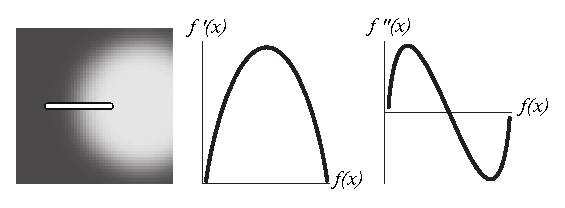
\includegraphics[width=0.75\textwidth]{images/g_cross_sampling}
		\label{fig:g_cross_sampling}
	}
	\subfigure[]
	{
		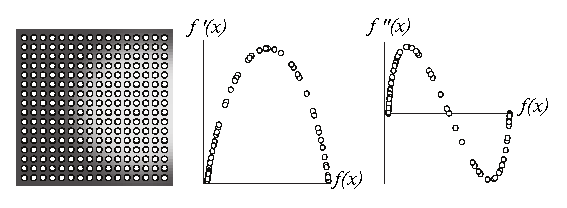
\includegraphics[width=0.75\textwidth]{images/g_full_sampling}
		\label{fig:g_full_sampling}
	}
	\caption{Comportamento de $ f'(x) $ e $ f''(x) $ em função de $ f(x) $ em: \ref{fig:g_cross_sampling} seção do volume com ocorrência de fronteira, \ref{fig:g_full_sampling} amostras por todo o volume~\cite{gordon}.}
	\label{fig:g_sampling}
\end{figure}

\begin{figure}[b]
	\centering
	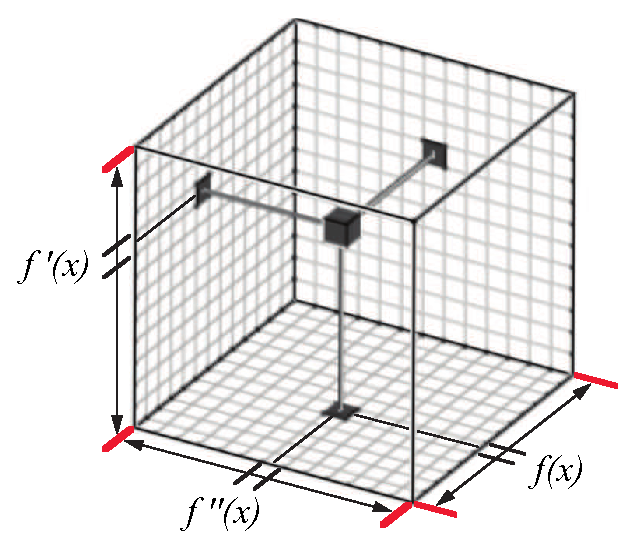
\includegraphics[width=0.5\textwidth]{images/g_histo3d}
	\caption{Histogramas 3D que armazena a relação entre $ f(x) $, $ f'(x) $ e $ f''(x) $~\cite{gordonms}.}
	\label{fig:g_histo3d}
\end{figure}
	
	Um histograma 3D de tamanho $ 256^{3} $ foi proposto para guardar a relação entre $ f(x) $, $ f'(x) $ e $ f''(x) $ independente de $x$. Cada eixo corresponde a uma das funções e os valores devem ser mapeados para o intervalo $ [0,255] $, como ilustra a Figura~\ref{fig:g_histo3d}. O histograma permite ainda gerar os histogramas 2D exibidos na Figura~\ref{fig:g_sampling}~\ref{fig:g_full_sampling}. Para obter um histograma 2D de $ f'(x) $ em função de $ f(x) $, acumula-se o histograma 3D na direção do eixo $ f''(x) $. Já para obter $ f''(x) $ em função de $ f(x) $, acumula-se na direção do eixo $ f'(x) $. Além disso, a partir dele é possível extrair as médias que serão utilizadas na geração da função de transferência, como será visto nas subseções~\ref{subsec:gordon.1d}~e~\ref{subsec:gordon.2d}.
	
	A Figura~\ref{fig:g_res} mostra os histogramas 2D acumulados para dois volumes de dados. No volume \quote{Turbine Blade} da Figura~\ref{fig:g_res}~\ref{fig:g_res_turbine}, observa-se que a intensidade é aproximadamente uma só. Dessa forma, espera-se que apenas uma fronteira seja identificada: aquela que separa a turbina de seu exterior. Essa expectativa é comprovada pelos histogramas acumulados. No primeiro histograma, três arcos se destacam, onde $ v_{min} = 0 $ (preto) e $ v_{max} = [130,190] $ (cinza claro).
	
	A justificativa para o intervalo dos valores finais dos arcos deve-se a uma pequena variação na intensidade da turbina. Contudo, o ponto de maior valor dos arcos é muito próximo, indicando uma única fronteira, próximo a $ 120 $. A mesma observação pode ser feita no segundo histograma, onde o ponto de inflexão médio das três curvas também é próximo a $ 120 $.
	
	Já na Figura~\ref{fig:g_res}~\ref{fig:g_res_engine}, três fronteiras são claramente demonstradas na fatia do volume \quote{Engine Block}: preto-branco, preto-cinza e cinza-branco. Como esperado, os histogramas também revelam essas fronteiras. O arco menor e mais forte indica a fronteira preto-cinza. O segundo arco menor representa a fronteira cinza-branco, enquanto o maior indica a fronteira preto-branco e, portanto, sobrepõem os dois outros arcos.
	
\begin{figure}[h]
	\centering
	\subfigure[]
	{
		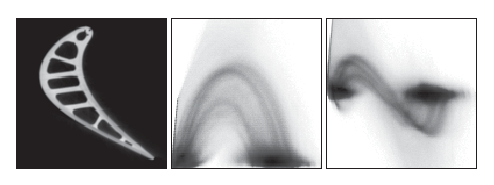
\includegraphics[width=0.75\textwidth]{images/g_res_turbine}
		\label{fig:g_res_turbine}
	}
	\subfigure[]
	{
		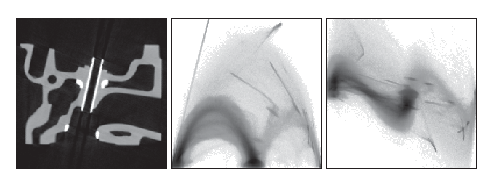
\includegraphics[width=0.75\textwidth]{images/g_res_engine}
		\label{fig:g_res_engine}
	}
	\caption{Esquerda: fatia do volume. Centro: Histograma 2D de $ f'(x) $ por $ f(x) $. Direita: Histograma 2D de $ f''(x) $ por $ f(x) $~\cite{gordon}.}
	\label{fig:g_res}
\end{figure}

\clearpage    
\section{Geração da Função de Transferência}
\label{sec:gordon.ft}
	A equação~\eqref{eq:boundary} deveria ser definida com 3 incógnitas, afinal o volume de dados pertence a um espaço tridimensional. No entanto, como as curvas exibidas na Figura~\ref{fig:g_functions} apenas são válidas na direção do gradiente, optou-se por mantê-las com apenas uma incógnita a fim de simplificar sua leitura. Portanto, ressalta-se que a coordenada $x$ não é alinhada a um eixo do volume, mas sim à direção do gradiente no ponto em que a função $f(x)$ é avaliada. Da mesma forma, a direção na notação das derivadas direcionais será omitida. Assim, a primeira e a segunda derivada de $f(x)$ na direção do gradiente são, respectivamente, $f'(x)$ e $f''(x)$ expressas nas equações \eqref{eq:first} e \eqref{eq:second}.
	\\
	
\begin{equation} \label{eq:first}
	g = f'(x) = \frac{v_{max} - v_{min}}{\sigma\sqrt{2\pi}}\ e^{-\frac{x^{2}}{2\sigma^{2}}}
\end{equation} \

\begin{equation} \label{eq:second}
	h = f''(x) = -\frac{x(v_{max} - v_{min})}{\sigma^{3}\sqrt{2\pi}}\ e^{-\frac{x^{2}}{2\sigma^{2}}}
\end{equation} \

	A função $f'(x)$ é uma gaussiana cujo desvio padrão é $\sigma$. Como a gaussiana tem pontos de inflexão em $\pm\sigma$, isso implica que $f''(x)$ atinge seus pontos extremos também em $\pm\sigma$. Observa-se pela Figura~\ref{fig:g_functions} que $2\sigma$ aproxima a distância entre $v_{max}$ e $v_{min}$, servindo assim como \quote{espessura} da fronteira. Cada volume possuirá um $\sigma$ diferente, que pode ser calculado uma vez que se saiba os valores máximos de $f'(x)$ e $f''(x)$. A partir do cálculo de $\sigma$ é possível extrair $x$ relacionando $f'(x)$ e $f''(x)$, como mostram as equações \eqref{eq:sigma} e \eqref{eq:x}.
	
\begin{equation} \label{eq:sigma}
	\sigma = \frac{f'(0)}{\sqrt{e}f''(-\sigma)}
\end{equation} \

\begin{equation} \label{eq:x}
	x = -\frac{\sigma^{2}f''(x)}{f'(x)}
\end{equation} \

	Isolar $x$ é importante pois ele é mais que uma posição do volume na direção do vetor gradiente. A posição indicada por $x$ é perpendicular à fronteira e relativa ao centro da mesma, ou seja, $|x|$ é a distância ao centro da fronteira. Em posse do valor de $ x $, fica mais fácil designar uma opacidade para cada voxel do volume, basta relacionar sua transparência de acordo com a sua distância à fronteira.
	
	A função par que decresce linearmente de $1$ a $0$ no intervalo $[0,\sigma]$ e permanece $0$ em $[\sigma, \infty]$ é provavelmente a forma mais intuitiva de relacionar a transparência com $x$. O volume se torna completamente opaco apenas nos pontos onde há ocorrência do centro exato de uma fronteira e vai perdendo essa opacidade linearmente até atingir uma região homogênea. Contudo, Kindlmann e Durkin designam ao usuário a tarefa de definir uma função de opacidade $ b(x) $ em função de $ x $.
	
	Através de $b(x)$ o usuário ganha um controle fino sobre o render final do volume, pois cabe a ele dizer como a fronteira deve ser visualizada. A Figura~\ref{fig:g_bx} mostra como diferentes opções de $b(x)$ podem afetar a visualização final. Nesse exemplo o volume é composto por duas esferas concêntricas de raios distintos. Percebe-se que apenas variando a função de opacidade é possível alternar entre: visualizar apenas a esfera de fora ou ambas, visualizar toda a fronteira ou apenas o lado interior da esfera que compõe a fronteira, ou até mesmo decidir entre uma transição suave ou abrupta.
	
\begin{figure}[h]
	\centering
	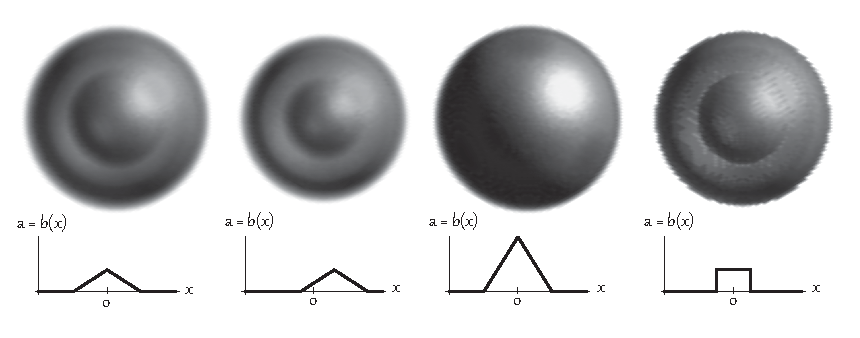
\includegraphics[width=1\textwidth]{images/g_bx}
	\caption{O impacto de diferentes funções de opacidade $b(x)$ na visualização de duas esferas concêntricas~\cite{gordon}.}
	\label{fig:g_bx}
\end{figure}

	Esse controle é especialmente importante quando as fronteiras de um volume não se comportam da forma ideal. Por exemplo, uma fronteira com o crescimento mais acentuado de um lado fará com que a distância $x$ seja deslocada. Neste caso, a correção desse deslocamento se torna muito mais simples se feita em $b(x)$ ao invés de $f(x)$. O usuário continua livre de ter que inspecionar o volume em busca da fronteira, mesmo que o método seja apenas capaz de indicar sua proximidade.
	
\subsection{Função de Transferência 1D}
\label{subsec:gordon.1d}
%TODO SIMPLIFICAR
	Com a premissa de que os materiais têm propriedades físicas homogêneas e o modelo definido na Seção~\ref{sec:gordon.bound}, pode-se assumir também que os valores do volume nas fronteiras são sempre os mesmos e que, na média, o centro de uma fronteira pode ser atribuído a um único valor escalar. Isso fica claro na Figura~\ref{fig:g_sampling} onde foi encontrado um padrão para identificar as fronteiras em função de $v$.
	
	A equação~\eqref{eq:x} reescrita em função de $v$ é apresentada na equação~\eqref{eq:pv}, cujo significado pode ser interpretado como a distância média com que os voxels de valor $v$ se encontram do centro da fronteira mais próxima. Nela, $g(v)$ indica a média da primeira derivada na direção do gradiente sobre todos os voxels de valor $v$. Da mesma forma, $h(v)$ indica a média da segunda derivada na direção do gradiente sobre todas as ocorrências de $v$. Ambas as médias podem ser extraídas através do centroide da fatia do histograma 3D indexada por $ v $, como mostra a Figura~\ref{fig:g_hv}
	
\begin{figure}[h]
	\centering
	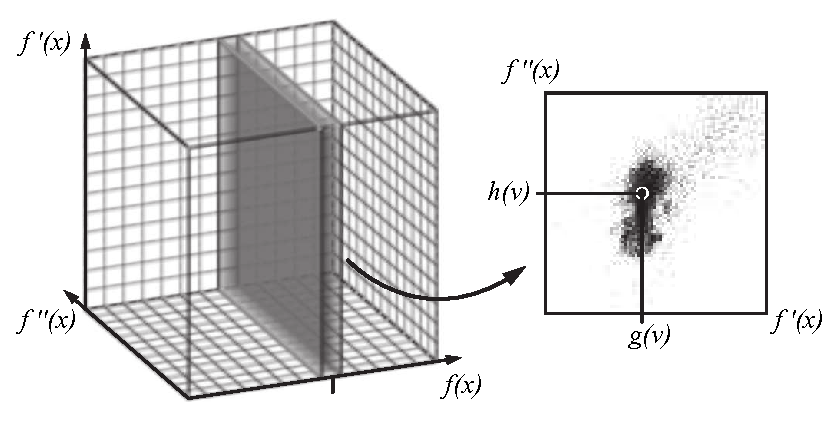
\includegraphics[width=1\textwidth]{images/g_hv}
	\caption{Fatia do histograma 3D, na posição $ v $~\cite{gordonms}.}
	\label{fig:g_hv}
\end{figure}

	As regiões homogêneas do volume deveriam possuir derivadas iguais a zero. No entanto, isso raramente acontece na prática. Para lidar com esse ruído, um threshold é inserido na equação~\eqref{eq:pv}. Não é fornecido nenhuma forma precisa de se obter $ g_{thresh} $. Apenas é sugerido que se o usuário for capaz de encontrar um valor escalar superior à derivada \quote{ambiente} do volume, a fórmula de $ p(v) $ será mais precisa.

\begin{equation} \label{eq:pv}
	p(v) = -\frac{\sigma^{2}h(v)}{max(g(v) - g_{thresh}, 0)}
\end{equation} \

	Como explicado previamente, $\sigma$ é obtido em função dos valores extremos de $f'(x)$ e $f''(x)$. Então, ele também precisa ser reformulado em função de $v$. O cálculo de $\sigma$ utilizando os máximos globais do volume pode distorcer todas as distâncias médias, por causa de ruído. Assim, os valores extremos utilizados devem ser os máximos dentre os valores médios: $g(v)_{max}$ e $h(v)_{max}$, como na equação~\eqref{eq:sigmav}. Uma forma mais equilibrada de obter o $\sigma$ é utilizar também o extremo mínimo da segunda derivada direcional, como demonstrado na equação~\eqref{eq:sigmav2}.
	
\begin{equation} \label{eq:sigmav}
	\sigma = \frac{g(v)_{max}}{\sqrt{e}\ h(v)_{max}}
\end{equation} \

\begin{equation} \label{eq:sigmav2}
	\sigma = \frac{2\ g(v)_{max}}{\sqrt{e}\ (h(v)_{max} - h(v)_{min})}
\end{equation} \

	Então, unindo as equações~\eqref{eq:x}~e~\eqref{eq:pv}, a função de transferência 1D é dada pela equação abaixo:
	
\begin{equation} \label{eq:alpha}
	\alpha(v) = b(p(v))
\end{equation} \

	As imagens abaixo mostram resultados para 3 volumes: molécula \quote{Bucky Ball}, \quote{Nucleon} e uma ressonância magnética da cabeça de um indivíduo. A Figura~\ref{fig:g_res_slices_1d} exibe fatias dos volumes, com o intervalo de intensidades mapeado entre preto e branco. A Figura~\ref{fig:g_res_fts_1d} apresenta as funções de transferência obtidas para cada volume. Por fim, a Figura~\ref{fig:g_res_vis_1d} mostra a visualização do volume com a FT gerada.
	
%%% SLICE
\begin{figure}[h]
	\centering
	\subfigure[\quote{Bucky Ball}]
	{
		
\includegraphics[width=0.3\textwidth]{images/g_bucky_slice}
		%\label{fig:}
	}
	\subfigure[\quote{Nucleon}]
	{
		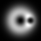
\includegraphics[width=0.3\textwidth]{images/g_nucleon_slice}
		%\label{fig:}
	}
	\subfigure[RM de uma cabeça]
	{
		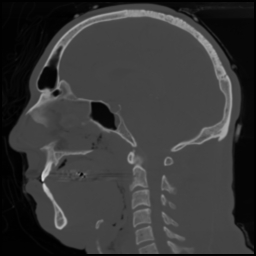
\includegraphics[width=0.3\textwidth]{images/g_vismale_slice}
		%\label{fig:}
	}
	\caption{Fatias dos volumes de dados.}
	\label{fig:g_res_slices_1d}
\end{figure}

%%% FT
\begin{figure}[]
	\centering
	\subfigure[\quote{Bucky Ball}]
	{
		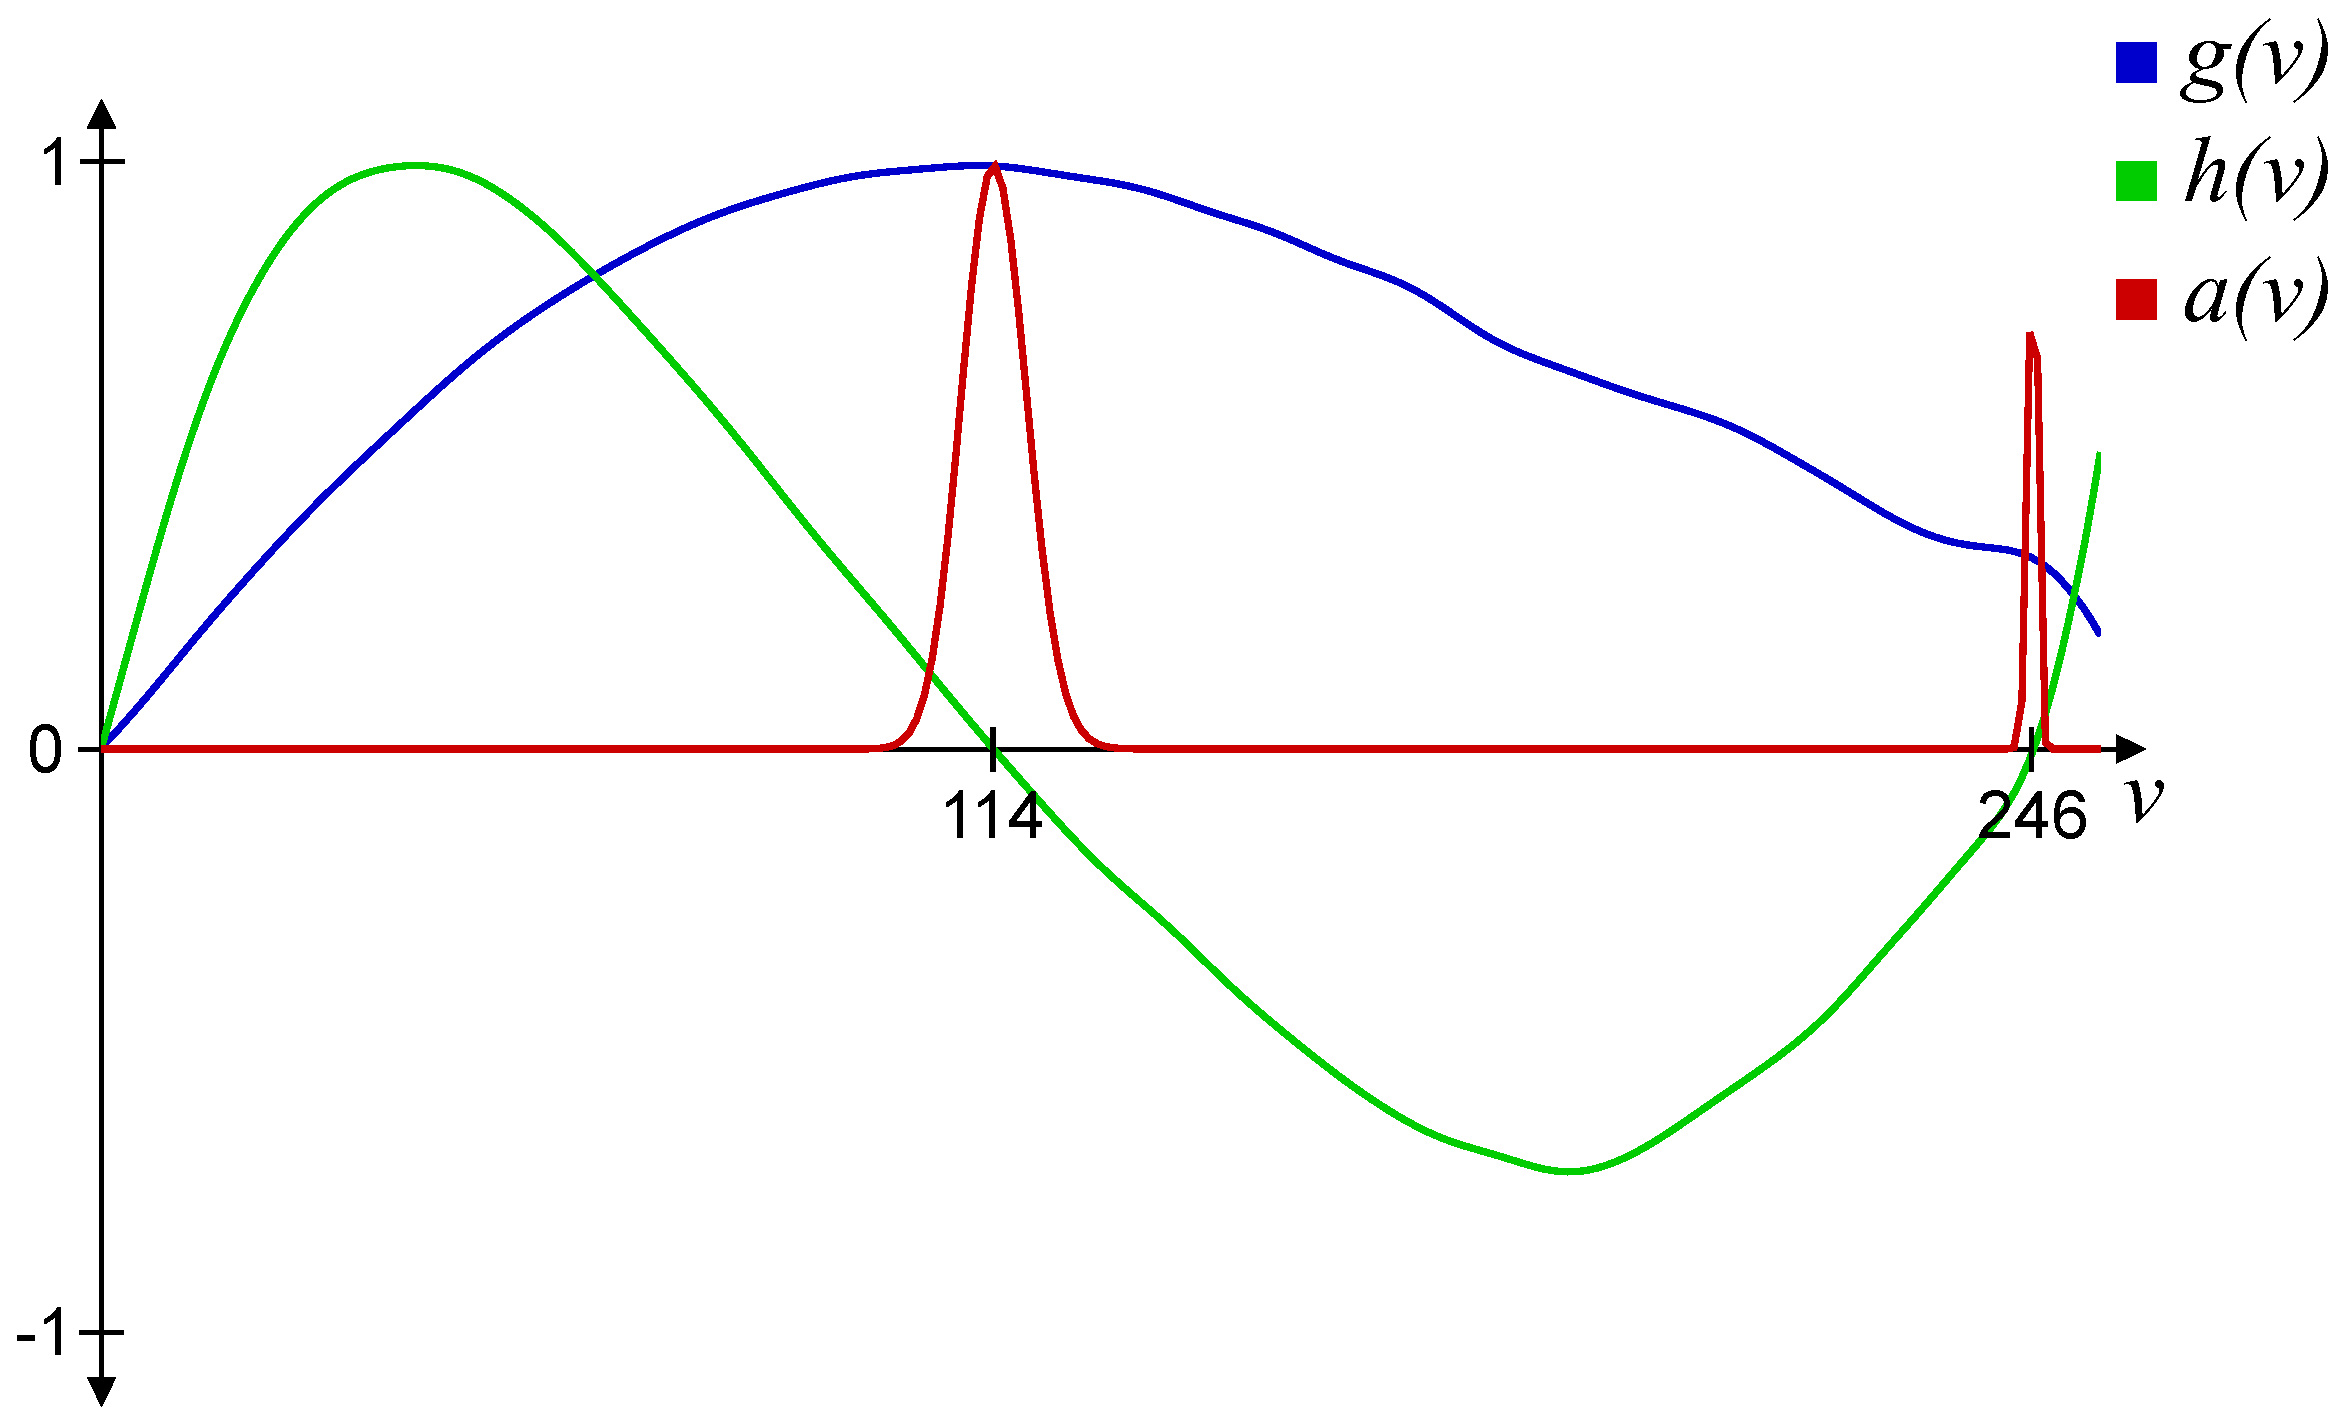
\includegraphics[width=0.7\textwidth]{images/g_bucky_ft}
		%\label{fig:}
	}
	\subfigure[\quote{Nucleon}]
	{
		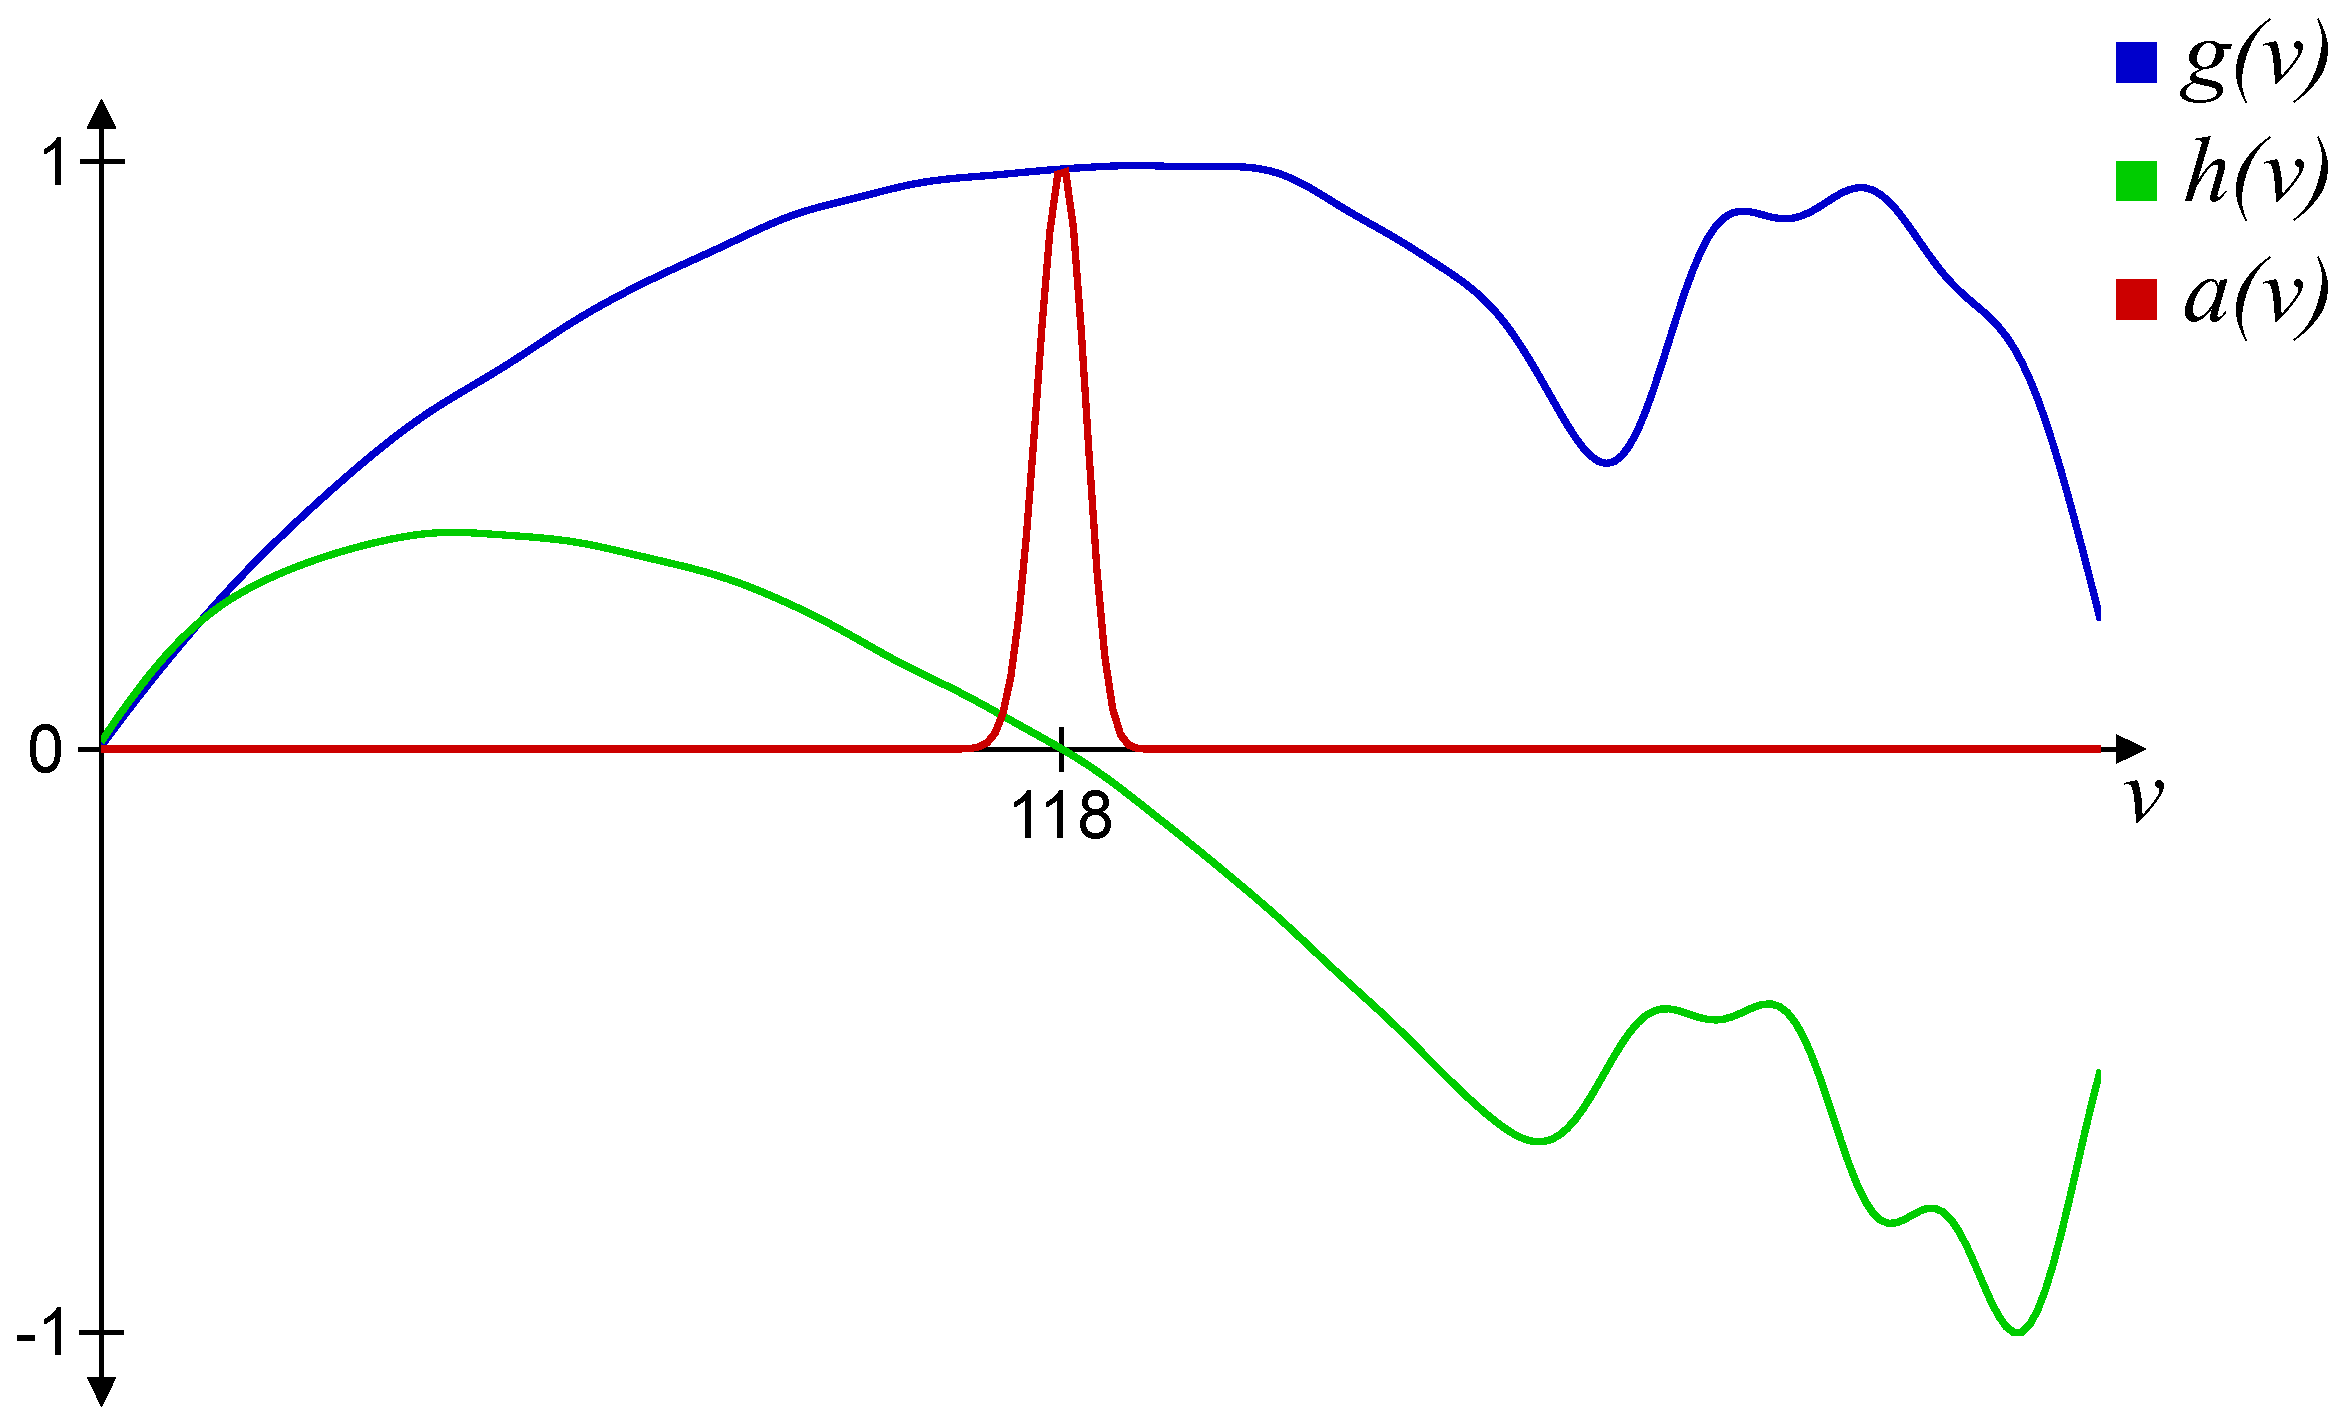
\includegraphics[width=0.7\textwidth]{images/g_nucleon_ft}
		%\label{fig:}
	}
	\subfigure[RM de uma cabeça]
	{
		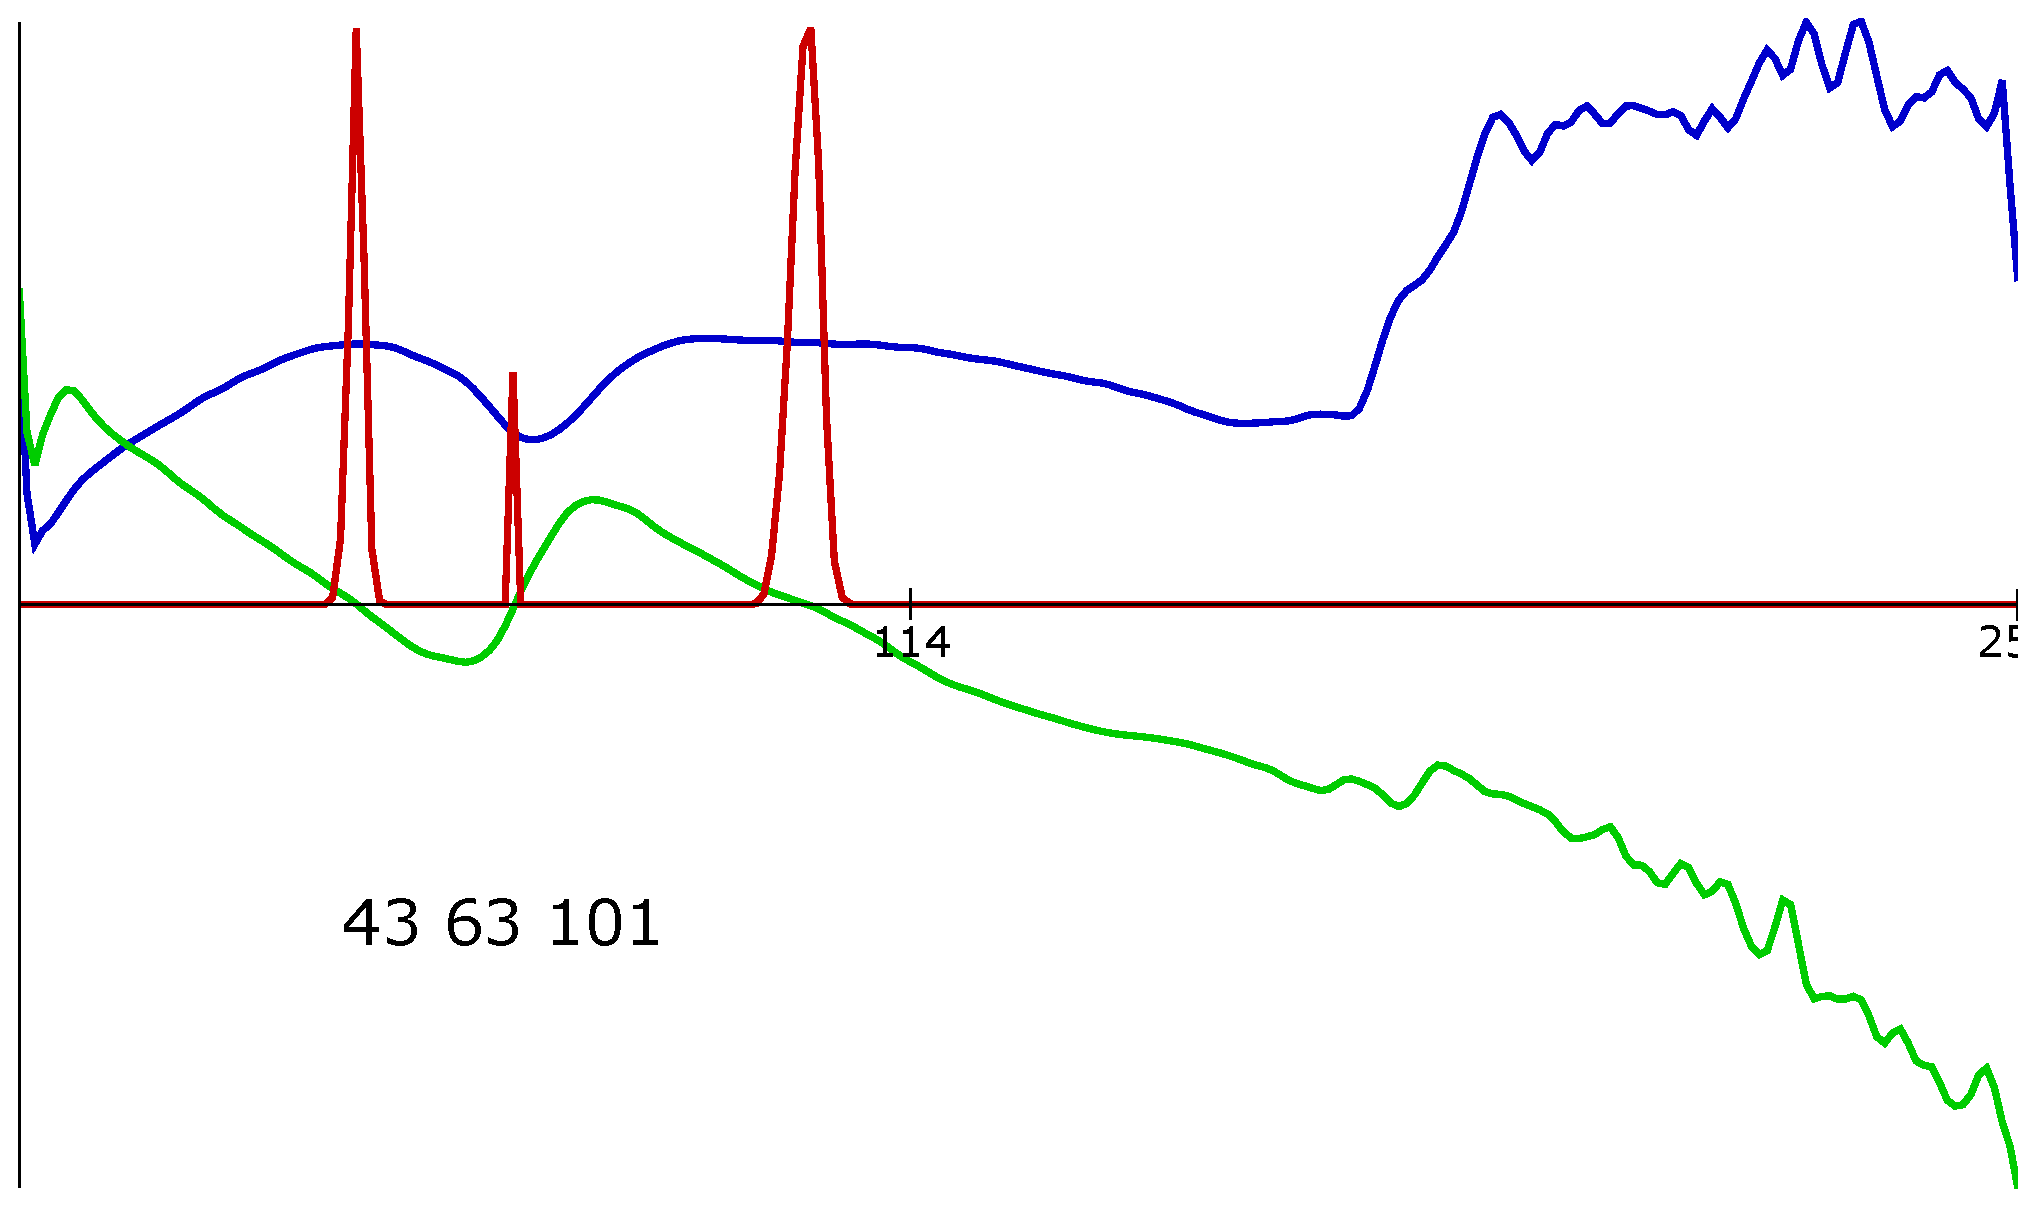
\includegraphics[width=0.7\textwidth]{images/g_vismale_ft}
		%\label{fig:}
	}
	\caption{Função de transferência 1D gerada para os volumes.}
	\label{fig:g_res_fts_1d}
\end{figure}

%%% ViSUAL
\begin{figure}[]
	\centering
	\subfigure[\quote{Bucky Ball}]
	{
		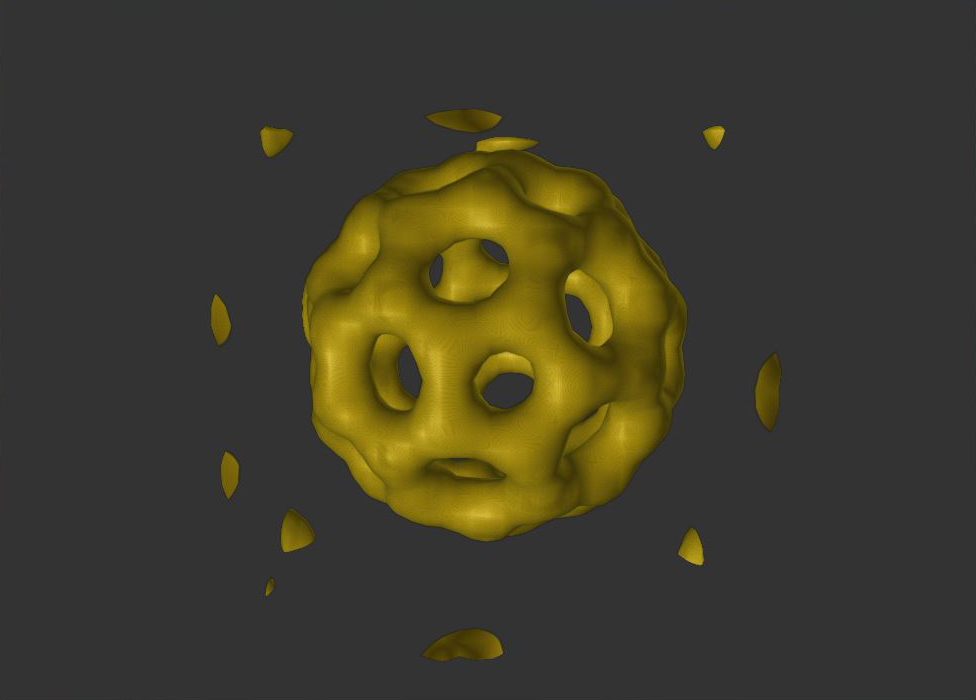
\includegraphics[width=0.5\textwidth]{images/g_bucky}
		%\label{fig:}
	}
	\subfigure[\quote{Nucleon}]
	{
		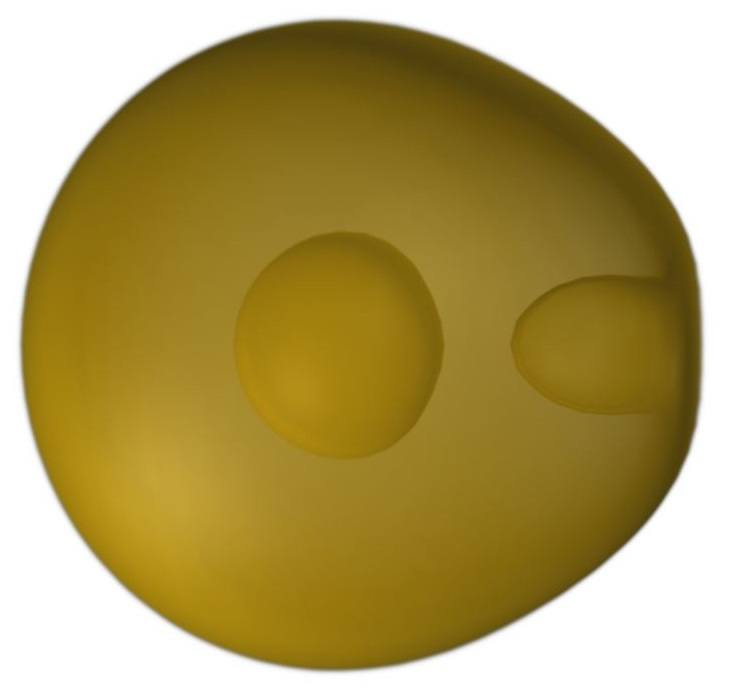
\includegraphics[width=0.5\textwidth]{images/g_nucleon}
		\label{fig:g_nucleon_1d}
	}
	\subfigure[RM de uma cabeça]
	{
		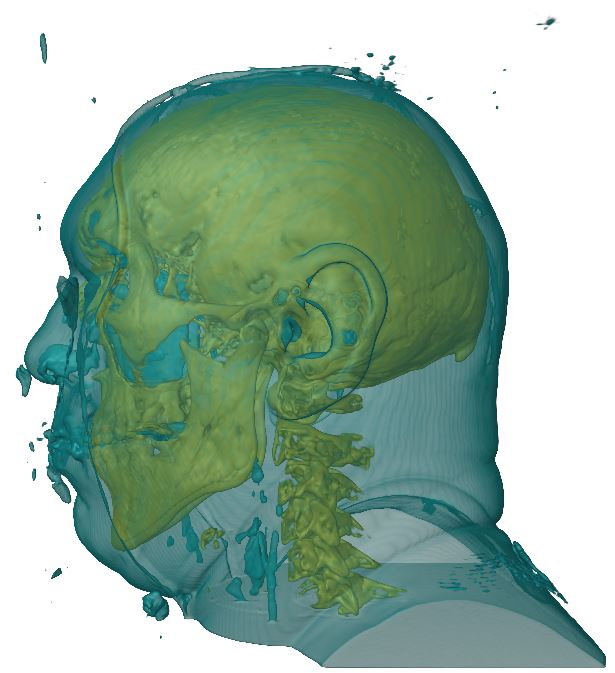
\includegraphics[width=0.5\textwidth]{images/g_vismale}
		%\label{fig:}
	}
	\caption{Visualização dos volumes com FT1D.}
	\label{fig:g_res_vis_1d}
\end{figure}

\clearpage
%%\newpage
\subsection{Função de Transferência 2D}
\label{subsec:gordon.2d}
	Uma função de transferência 2D designa opacidade não só em função da intensidade do volume, mas também em função de um segundo parâmetro. O uso dessa segunda dimensão tende a diminuir a sobreposição de intervalos das fronteiras. No entanto, ao mesmo tempo que torna a FT mais precisa, a adição de uma nova dimensão também dificulta muito sua especificação de forma manual. Então, 
	\textit{Kindlmann e Durkin}~\cite{gordon} estenderam o método descrito até aqui, utilizando a primeira derivada para compor a FT2D.
	
	O cálculo de $\sigma$ permanece inalterado, como na equação~\eqref{eq:sigmav2}. A distância média à fronteira, porém, precisa ser reescrita também em função da primeira derivada. Logo, $p(v)$ é substituída por $p(v,g)$ descrita na equação~\eqref{eq:pvg}. O termo $h(v,g)$ é a segunda derivada média para cada ocorrência de escalar $v$ e primeira derivada $g$. Assim como na versão 1D, esse valor médio também pode ser extraído do histograma 3D, como indica a Figura~\ref{fig:g_hvg}. A função de transferência 2D final é então representada pela função $ \alpha(v, g) $, descrita na equação~\eqref{eq:alphavg}.
    
\begin{figure}[h]
	\centering
	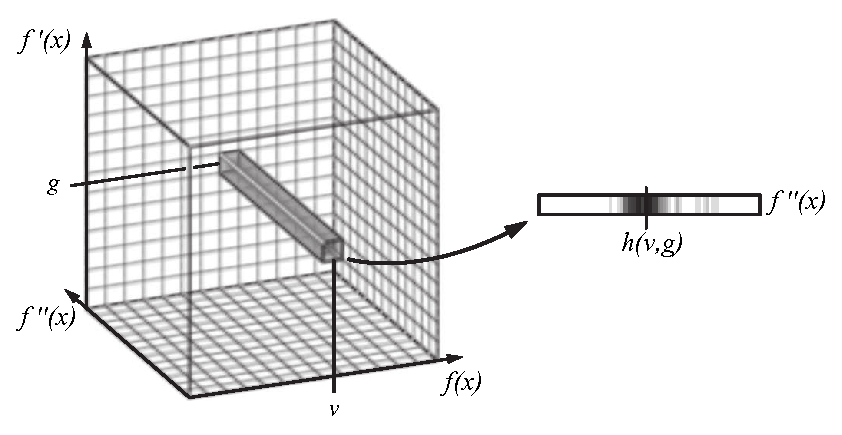
\includegraphics[width=1\textwidth]{images/g_hvg}
	\caption{Seção do histograma 3D indexado por $ v $ e $ g $~\cite{gordonms}.}
	\label{fig:g_hvg}
\end{figure}
    
\begin{equation} \label{eq:pvg}
	p(v,g) = -\frac{\sigma^{2}h(v,g)}{max(g - g_{thresh}, 0)}
\end{equation} \

\begin{equation} \label{eq:alphavg}
	\alpha(v, g) = b(p(v, g))
\end{equation} \

	As imagens abaixo mostram resultados para os mesmos 3 volumes da seção anterior: molécula \quote{Bucky Ball}, \quote{Nucleon} e uma ressonância magnética da cabeça de um indivíduo. A Figura~\ref{fig:g_res_vis_2d} exibe as visualizações dos volumes a partir das funções de transferência que foram obtidas, exibidas na Figura~\ref{fig:g_res_fts_2d}
	
%%% ViSUAL
\begin{figure}[h]
	\centering
	\subfigure[\quote{Bucky Ball}]
	{
		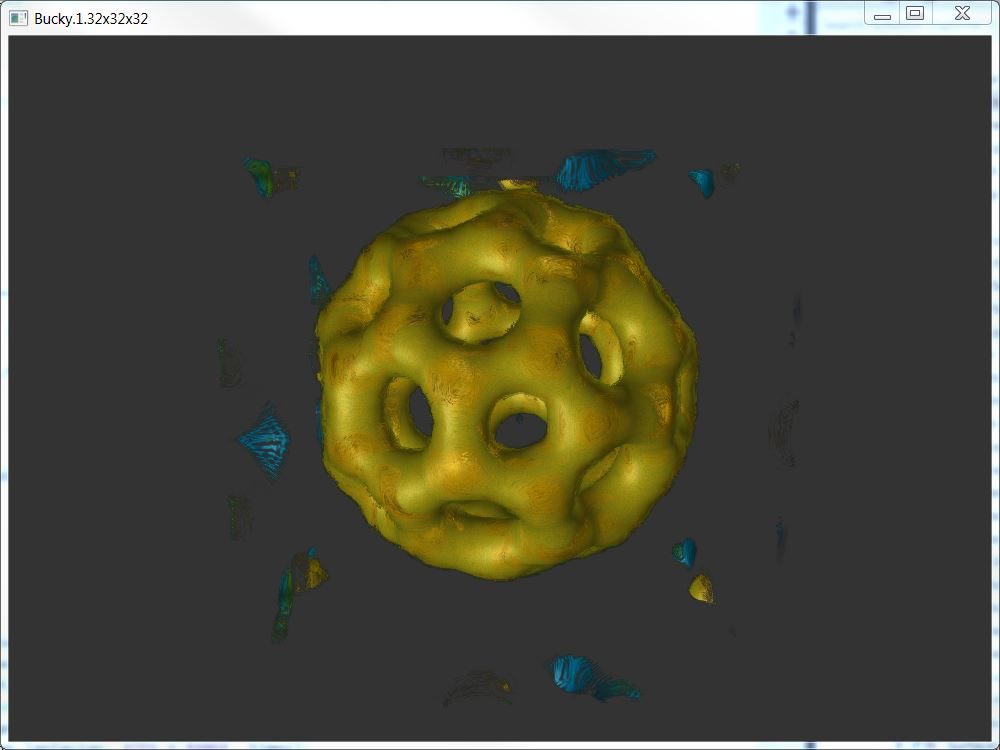
\includegraphics[width=0.5\textwidth]{images/g_bucky_2d}
		%\label{fig:}
	}
	\subfigure[\quote{Nucleon}]
	{
		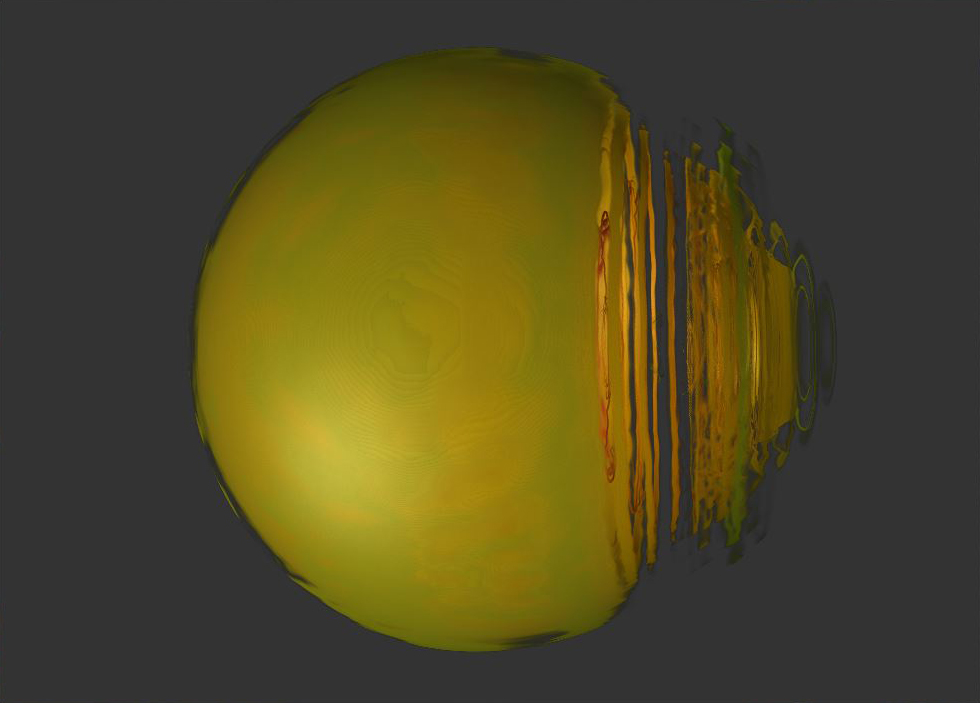
\includegraphics[width=0.5\textwidth]{images/g_nucleon_2d}
		%\label{fig:}
	}
	\subfigure[RM de uma cabeça]
	{
		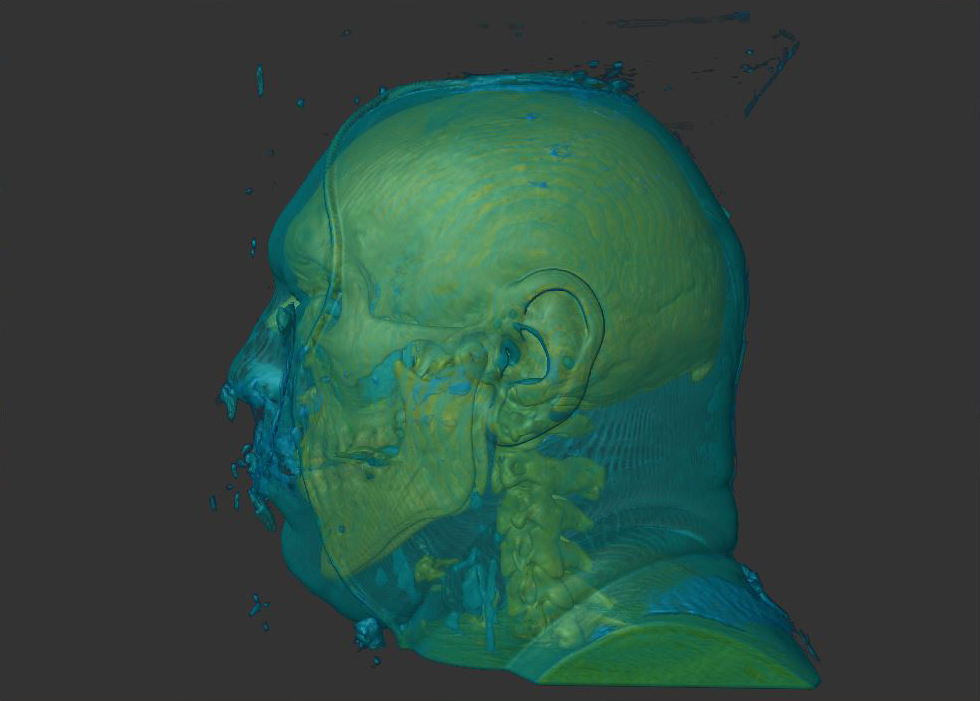
\includegraphics[width=0.5\textwidth]{images/g_vismale_2d}
		%\label{fig:}
	}
	\caption{Visualização dos volumes com FT2D}
	\label{fig:g_res_vis_2d}
\end{figure}

%%% FT
\begin{figure}[]
	\centering
	\subfigure[\quote{Bucky Ball}]
	{
		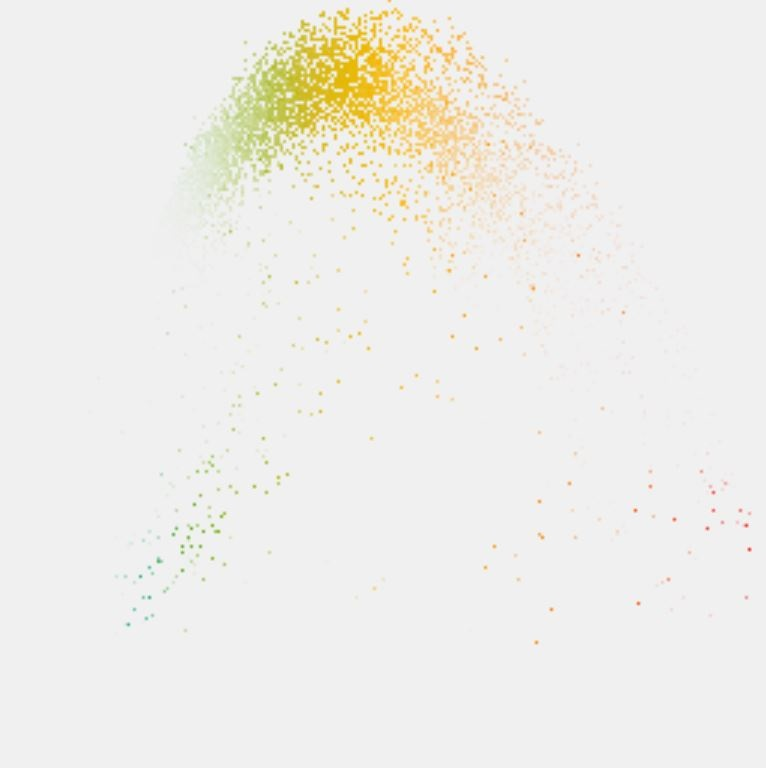
\includegraphics[width=0.5\textwidth]{images/g_bucky_ft_2d}
		%\label{fig:}
	}
	\subfigure[\quote{Nucleon}]
	{
		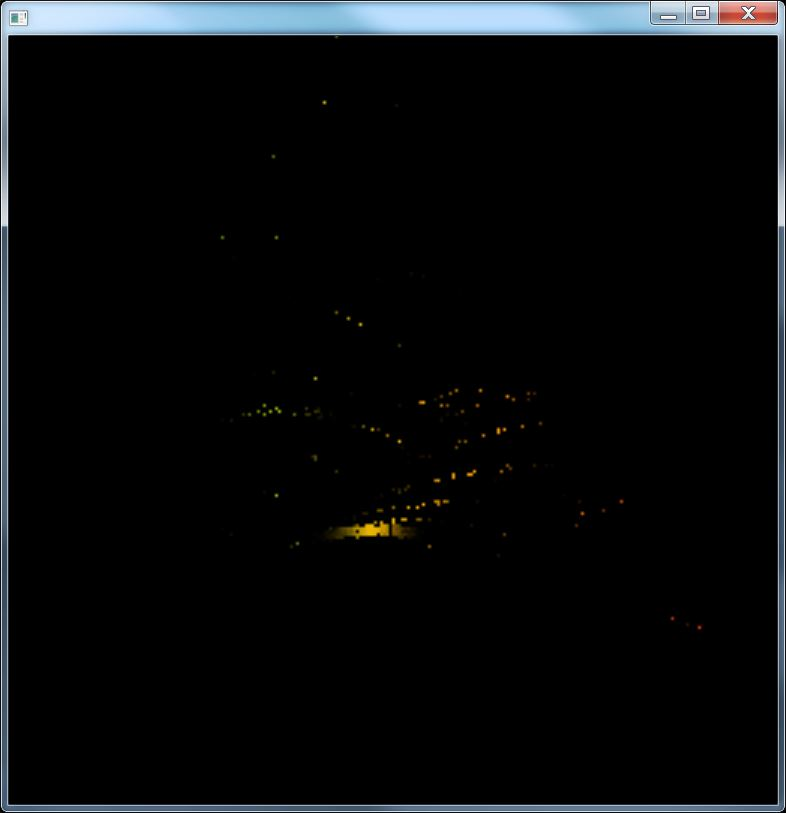
\includegraphics[width=0.5\textwidth]{images/g_nucleon_ft_2d}
		\label{fig:g_nucleon_2d}
	}
	\subfigure[RM de uma cabeça]
	{
		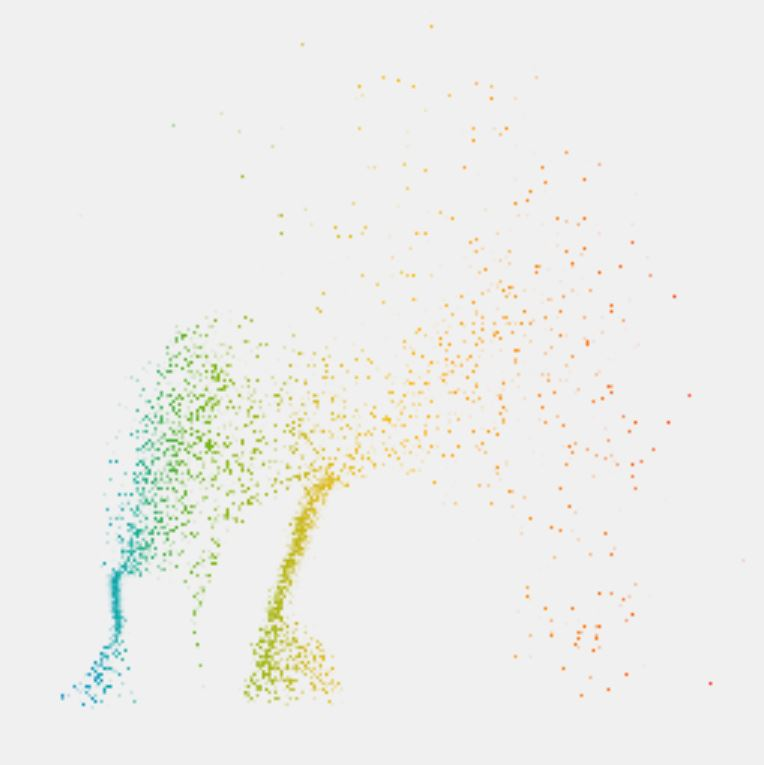
\includegraphics[width=0.5\textwidth]{images/g_vismale_ft_2d}
		%\label{fig:}
	}
	\caption{Função de transferência 2D gerada para os volumes.}
	\label{fig:g_res_fts_2d}
\end{figure}

\clearpage
\section{Avaliação do Método}
\label{sec:gordon.aval}
	O método de \textit{Kindlmann e Durkin}~\cite{gordon} identifica bem as fronteiras que ocorrem em um volume. Os arcos de seu histograma acumulado permitem ver quantas fronteiras bem definidas existem, além de indicar o intervalo de valores no qual a fronteira varia. Nos casos em que os arcos não são tão distintos, o modelo matemático da função de transferência ainda é capaz de proporcionar bons resultados.
	
	No entanto, quando os arcos se cruzam no histograma, o modelo matemático não é capaz de distinguir entre as fronteiras existentes no intervalo de valores sobrepostos. Isso pode acarretar em uma função de transferência que não destaca as fronteiras corretamente. Nesses casos, uma solução pode ser o uso de funções de transferência 2D, que melhoraram a classificação dos valores quanto às fronteiras. Contudo, como observado por \textit{Sereda et al.}~\cite{sereda1}, nem sempre o aumento na dimensão da FT resolve essa sobreposição.
	
	Além disso, não há garantia de que o uso de uma função de transferência 2D não resultará em uma visualização pior que a obtida com uma 1D, como visto no volume \quote{Nucleon}: Figuras~\ref{fig:g_res_fts_1d}~\ref{fig:g_nucleon_1d} e \ref{fig:g_res_fts_2d}~\ref{fig:g_nucleon_2d}. Dessa forma, a função de transferência 1D se torna preferível. Por ser mais intuitiva e fácil de manipular, ela permite que o usuário faça correções quando a visualização não estiver adequada.
	
	Ainda perseguindo o objetivo de que a tarefa do usuário deve ser facilitada, é preciso ressaltar que o threshold utilizado nas equações \eqref{eq:pv} e \eqref{eq:pvg} é um parâmetro trabalhoso de se escolher. Em alguns volumes, o valor necessário é tão pequeno que pode ser desconsiderado em troca de utilizar uma função $ b(x) $ estreita. Contudo, pode ser preciso um threshold alto para que a visualização permita uma compreensão adequada do volume. Por outro lado, o uso de um $ g_{thresh} $ grande, sem necessidade, pode impedir a visualização de fronteiras mais fracas, isto é, de menor $ g $. A Figura~\ref{fig:g_res_thresh} mostra a função de transferência e a visualização do volume \quote{Bonsai} sem threshold e com threshold.
	
	Ao longo desta dissertação, descobriu-se que um valor bom é o equivalente ao menor vale na curva da primeira derivada média, $ g(v) $. Esta foi a regra utilizada para gerar os resultados de \textit{Kindlmann e Durkin}~\cite{gordon} e, nos volumes avaliados, não houve melhora significativa com a variação desse valor. No entanto, mais estudos devem ser feitos para definir um $ g_{thresh} $ garantidamente adequado.
	
\begin{figure}[h]
	\centering
	\subfigure[Função de transferência sem threshold]
	{
		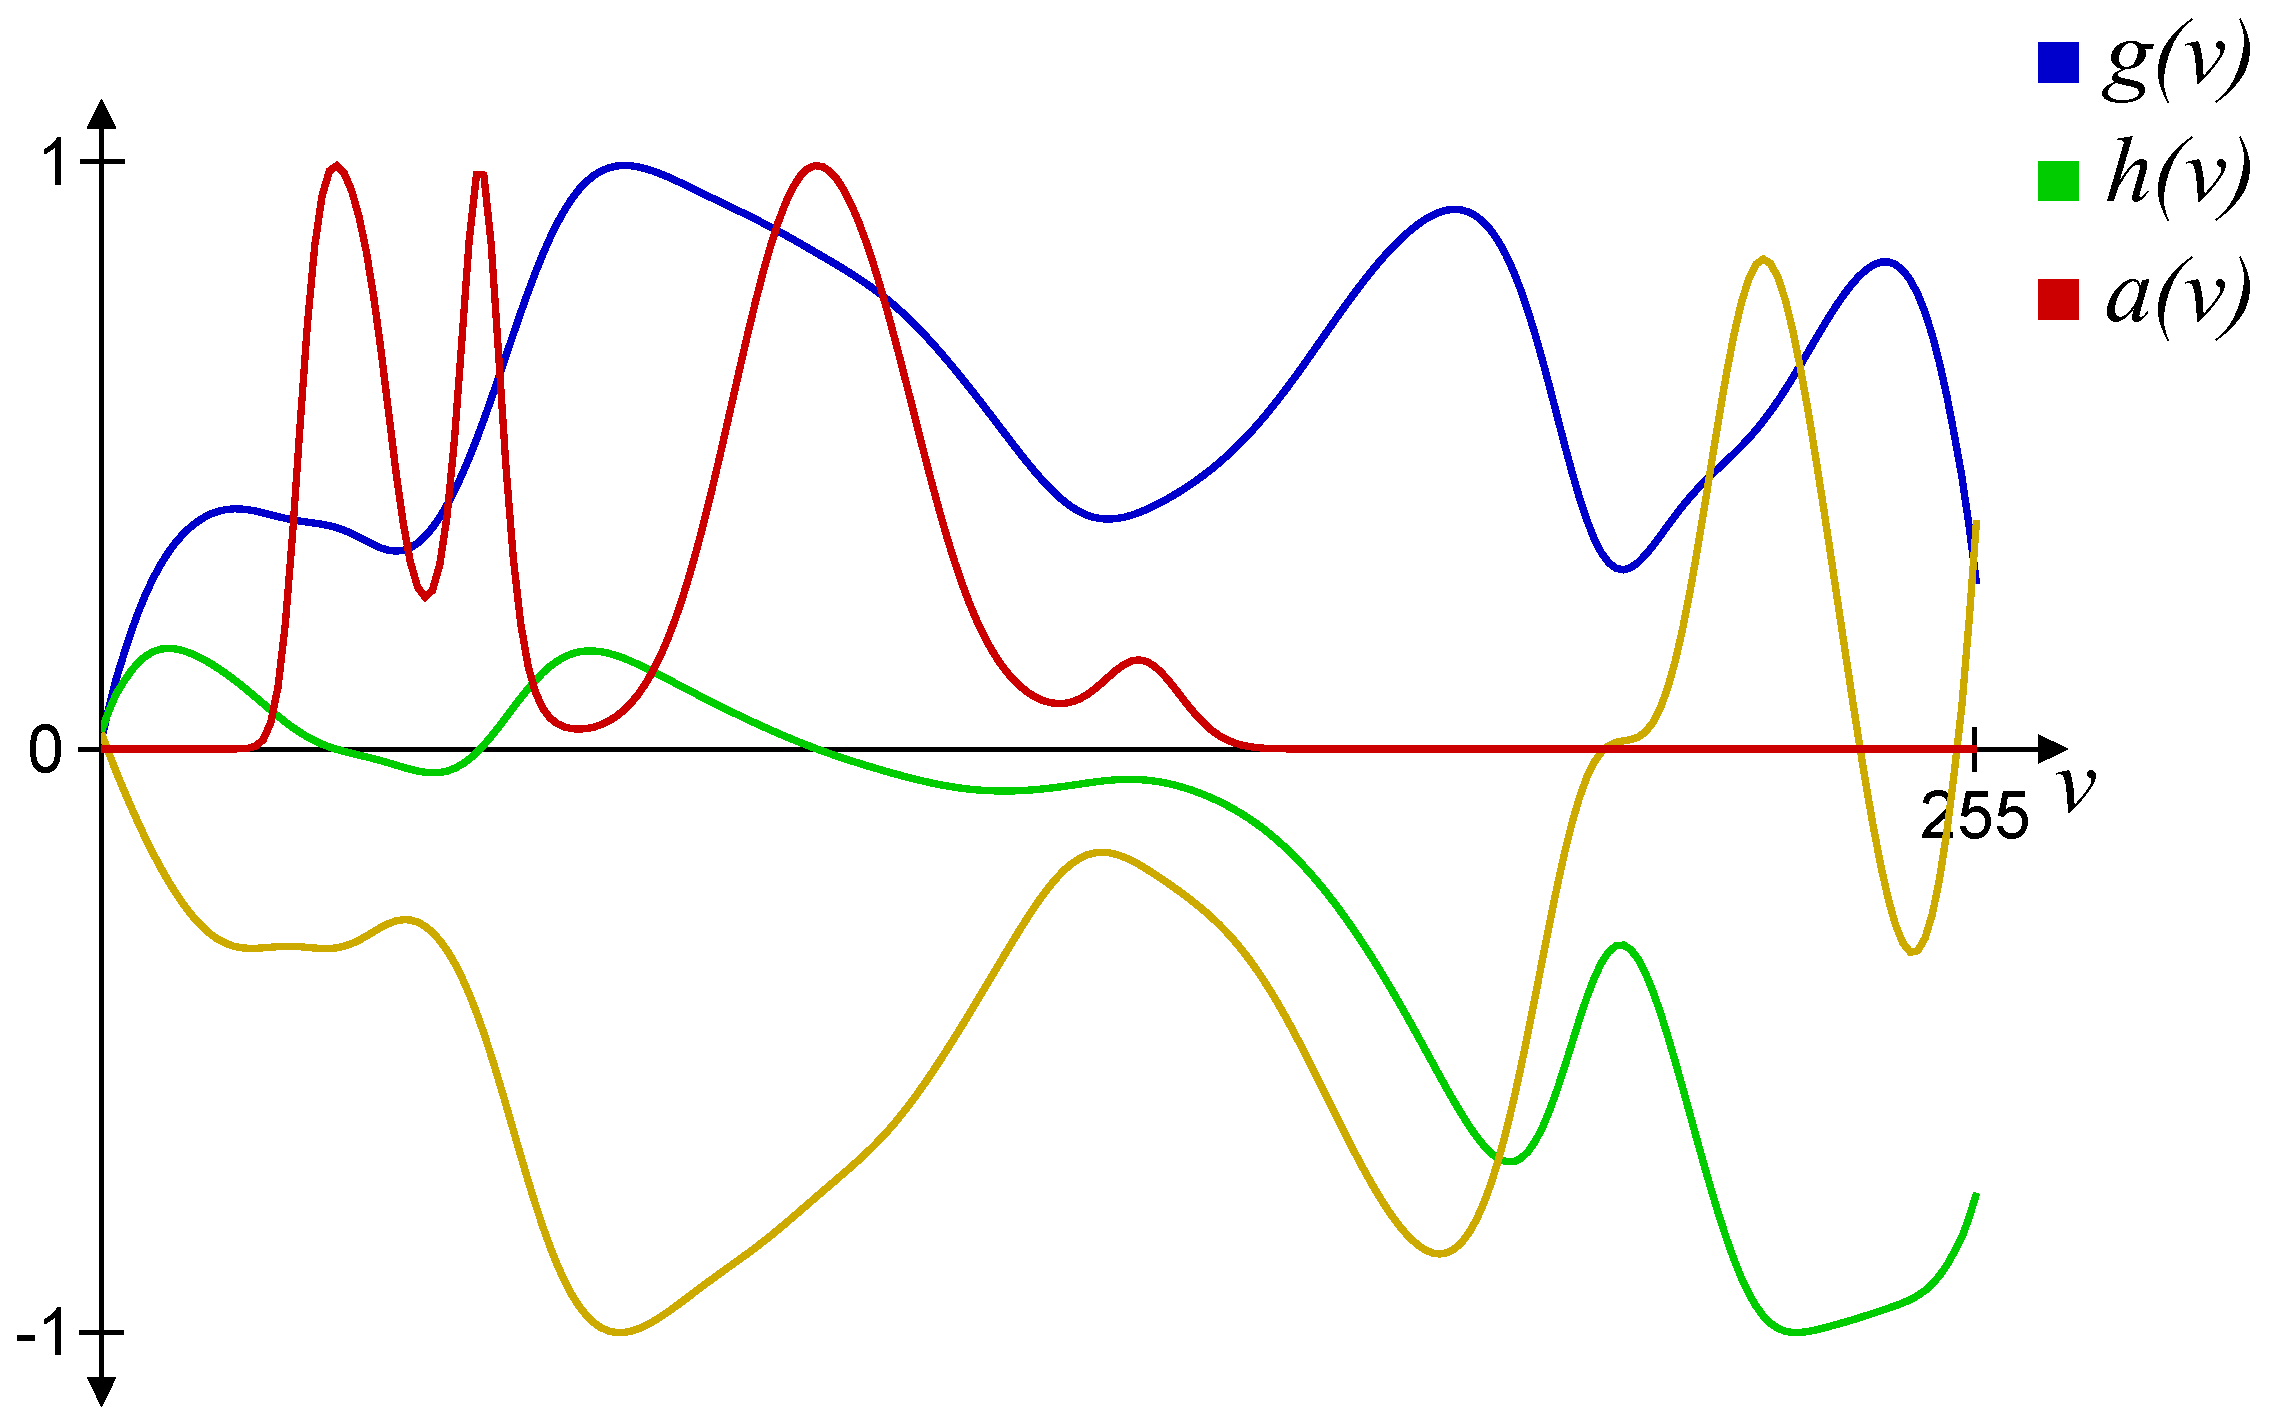
\includegraphics[width=0.7\textwidth]{images/g_bonsai_nothresh_ft}
		\label{fig:nothresh}
	}
	\subfigure[Função de transferência com threshold]
	{
		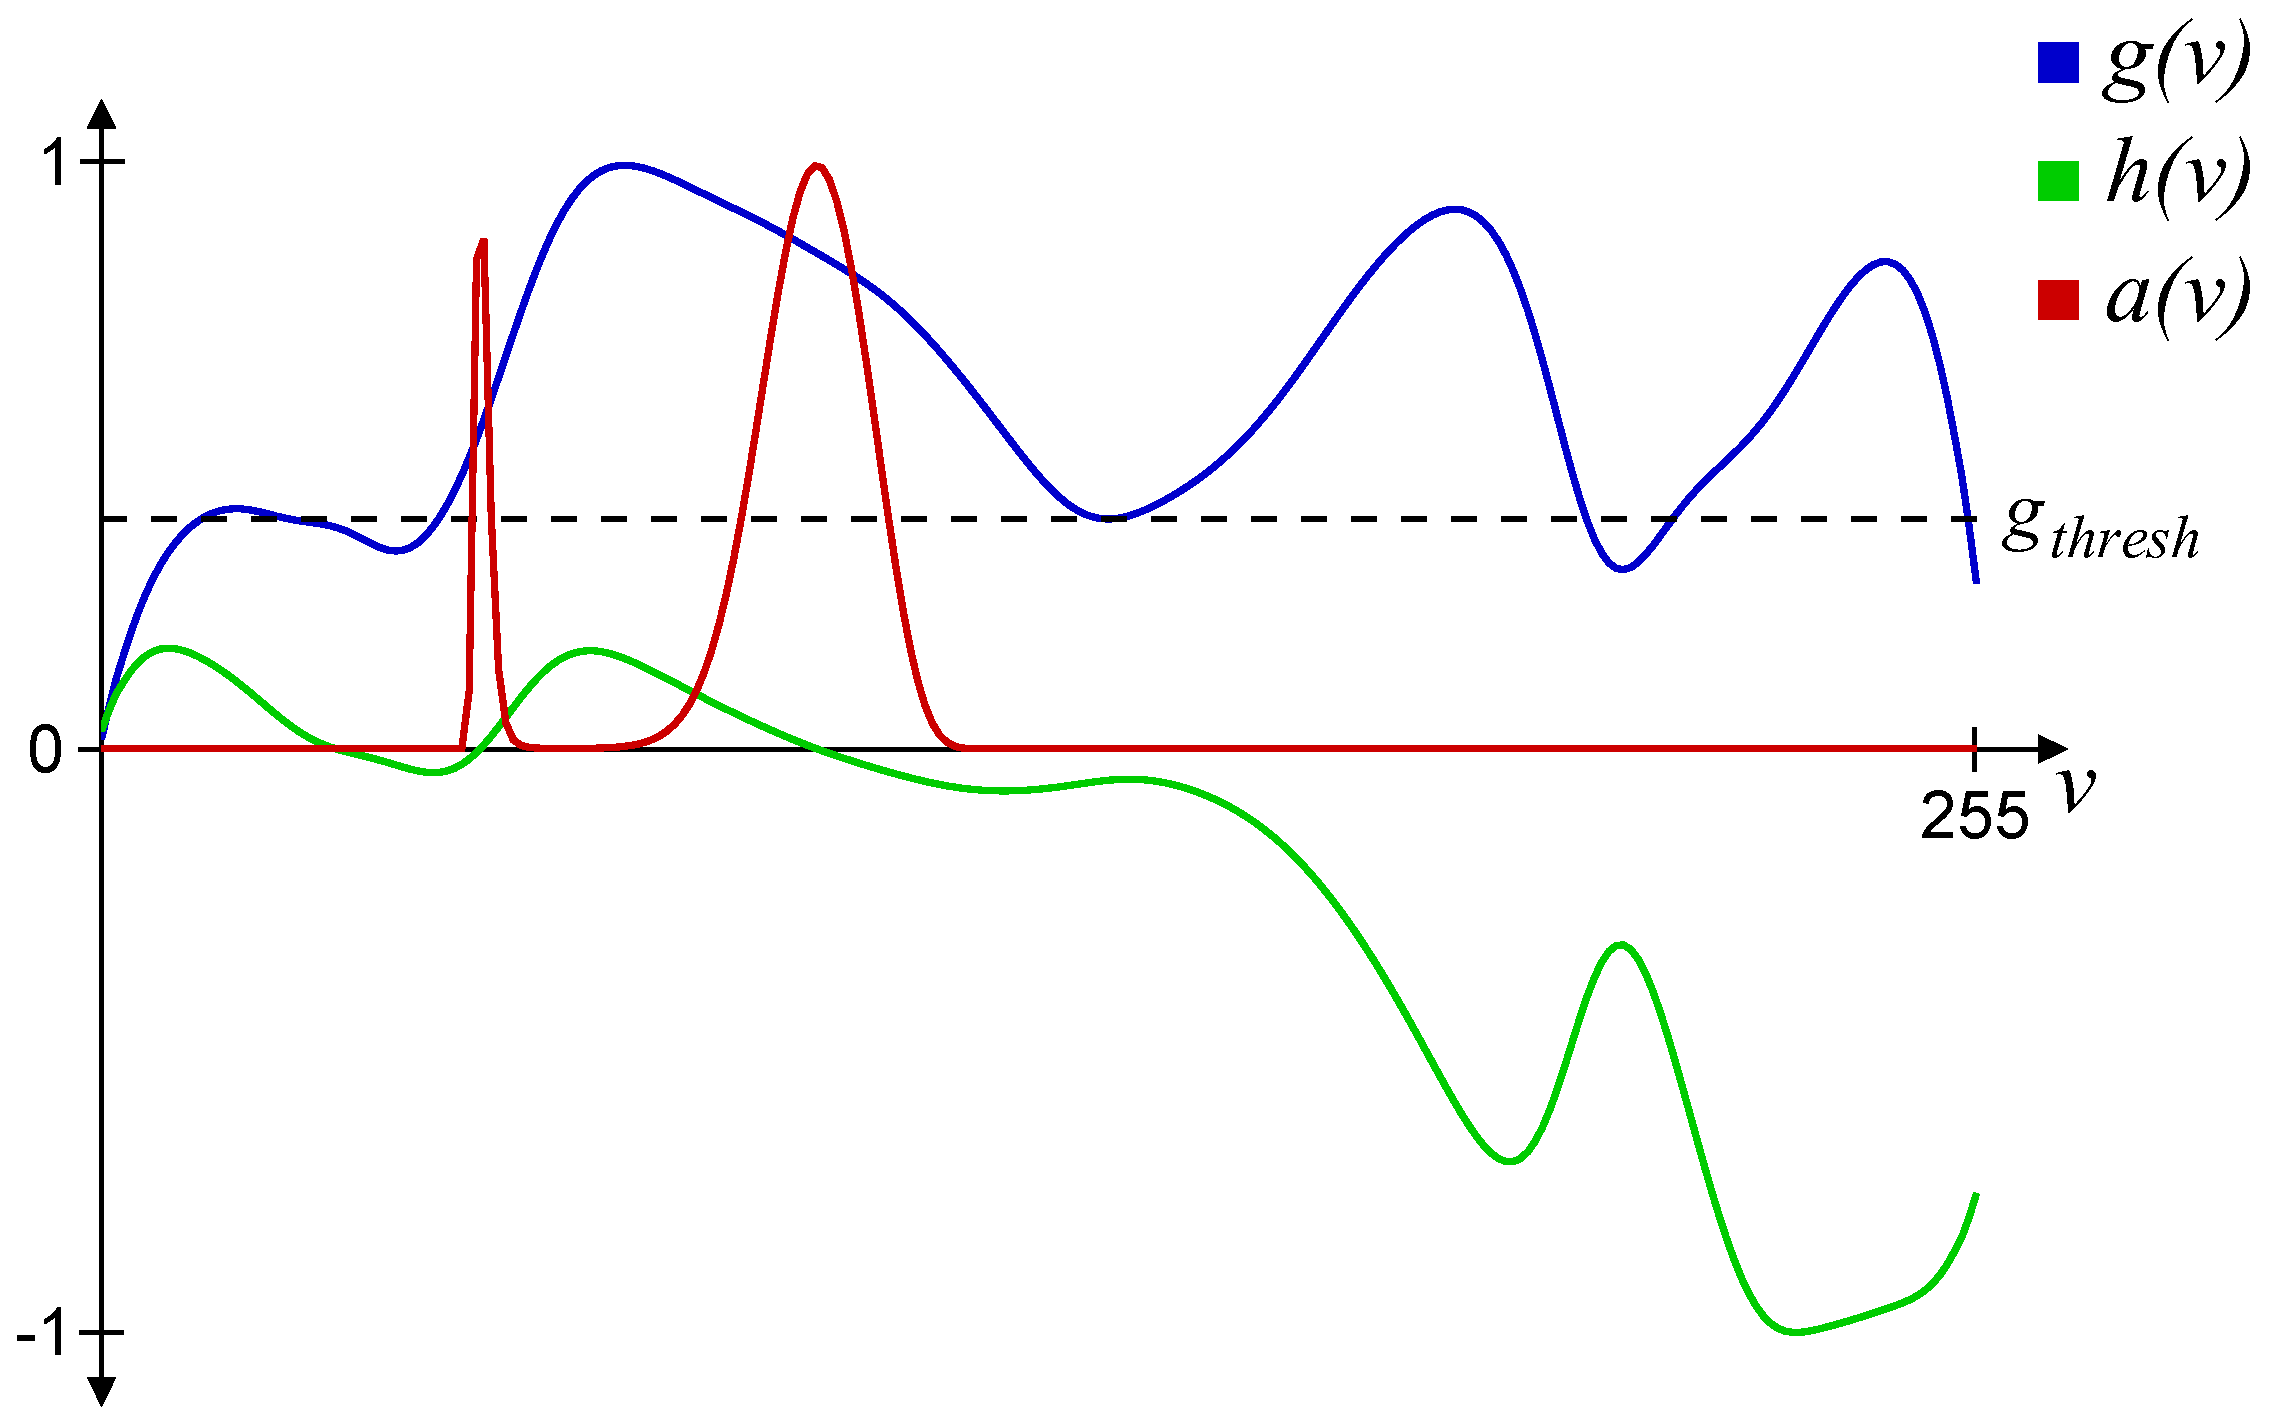
\includegraphics[width=0.7\textwidth]{images/g_bonsai_ft}
		\label{fig:thresh}
	}
	\subfigure[\quote{Bonsai} sem threshold]
	{
		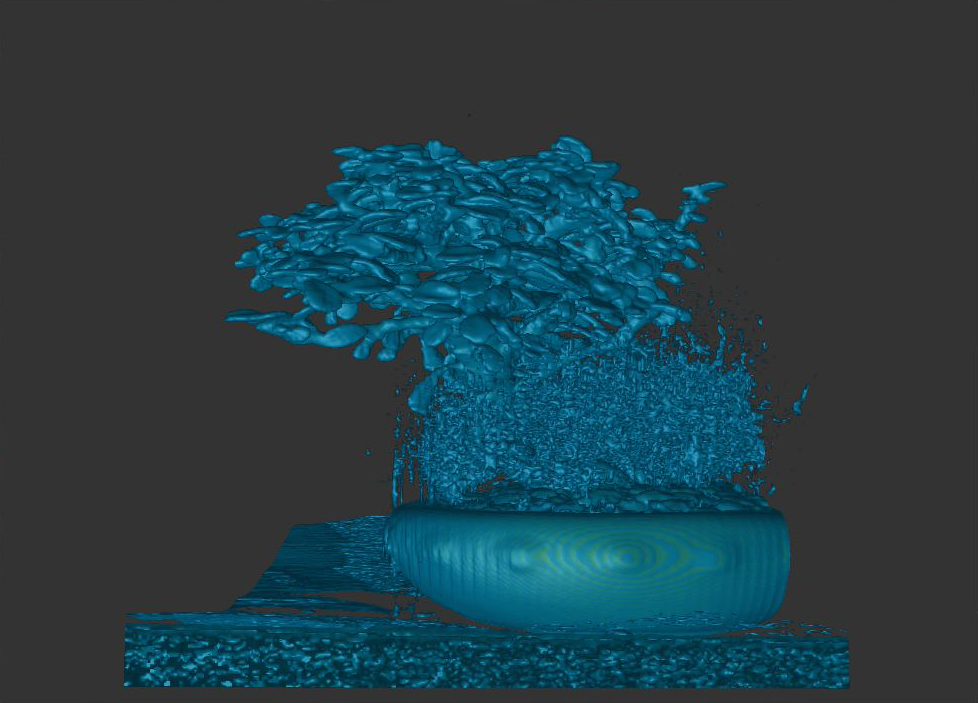
\includegraphics[width=0.47\textwidth]{images/g_bonsai_nothresh}
		\label{fig:nothresh_ft}
	}
	\subfigure[\quote{Bonsai} com threshold]
	{
		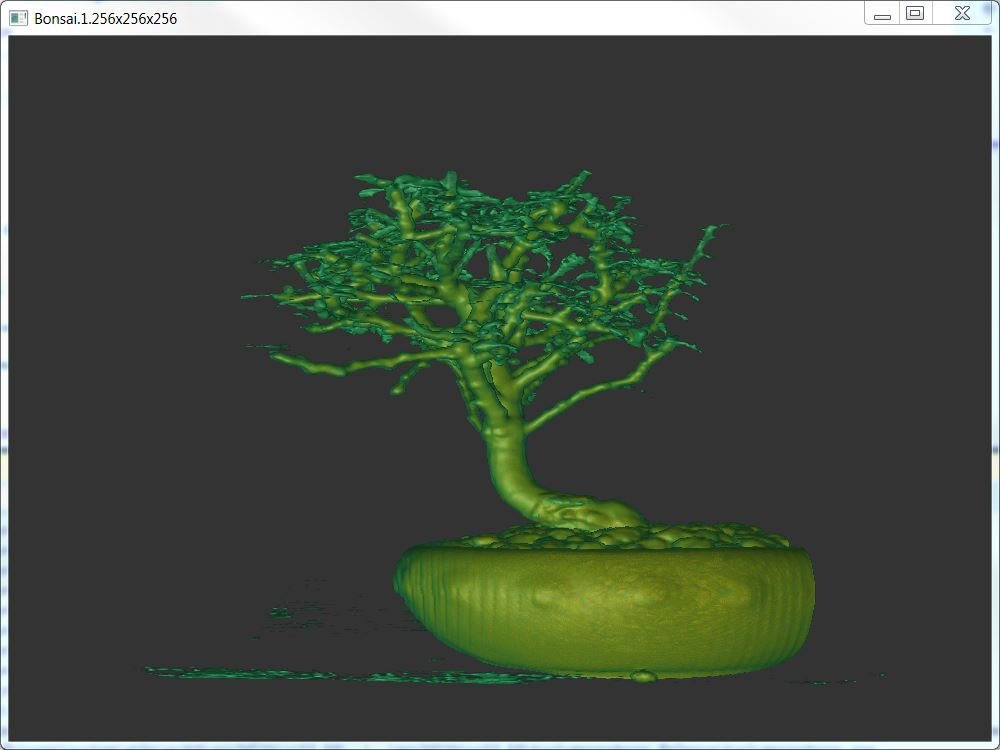
\includegraphics[width=0.47\textwidth]{images/g_bonsai}
		\label{fig:thresh_ft}
	}
	\caption{O impacto do $g_{thresh}$ na função de transferência.}
	\label{fig:g_res_thresh}
\end{figure}
	
	A solução para o valor do $ g_{thresh} $ emergiu da ideia de que $ g(v) $ pode conter um deslocamento em sua imagem, devido ao fato de que ela é composta pela média dos valores da primeira derivada quantizados no histograma. Esse é o motivo pelo qual se decidiu utilizar o menor vale como $ g_{thresh} $, pois indica a menor base de um possível arco.
	
    Uma análise mais profunda da equação~\eqref{eq:x}, repetida abaixo por comodidade, revela que $ f''(x) $ possui um peso maior que $ f'(x) $ na determinação de uma fronteira. Como visto nesse capítulo, o centro exato de uma fronteira é indicado por $ x = 0 $. Matematicamente, isso só ocorre quando $ f''(x) = 0 $ ou $ f'(x) $ tende a infinito. Dado o comportamento conhecido das funções $ f'(x) $ e $ f''(x) $, sabe-se que $ f''(x) $ assume $ 0 $ três vezes ao longo de x. No entanto, $ f'(x) $ nunca assume infinito.
    
\begin{equation} \label{eq:xpvg}
	x = -\frac{\sigma^{2}f''(x)}{f'(x)} \ \approx \ 
	p(v) = -\frac{\sigma^{2}h(v)}{max(g(v) - g_{thresh}, 0)}
\end{equation} \

	Um argumento válido é de que, na prática, $ f'(x) $ não precisa se aproximar tanto de $ \pm \infty $ para que a equação~\eqref{eq:xpvg} resulte em um $ x $ suficientemente próximo de zero. Basta atingir um valor grande o suficiente para aproximar $ x $ de zero, independente do valor de $ f''(x) $. No entanto, tal resultado necessitaria de uma descontinuidade em $ f(x) $ que não é compatível com o modelo de fronteira assumido. Por isso, $ f''(x) $ desempenha um papel muito mais importante na definição de uma fronteira.
	
	O problema dessa abordagem se torna mais evidente uma vez que $ x $ é aproximado por valores médios através da função $ p(v) $. Um deslocamento na imagem de $ g(v) $ não altera o valor $ v $ que identifica a fronteira, uma vez que os valores máximos de $ g(v) $ e $ g(v) + c $ ocorrem na mesma posição. No entanto, o mesmo não é verdade para a função $ h(v) $, como mostra a Figura~\ref{fig:g_shift}. Isso porque as equações $ h(v) = 0 $ e $ h(v) + c = 0 $ são satisfeitas em valores $ v $ distintos.
	
\begin{figure}[h]
	\centering
	\subfigure[] {
		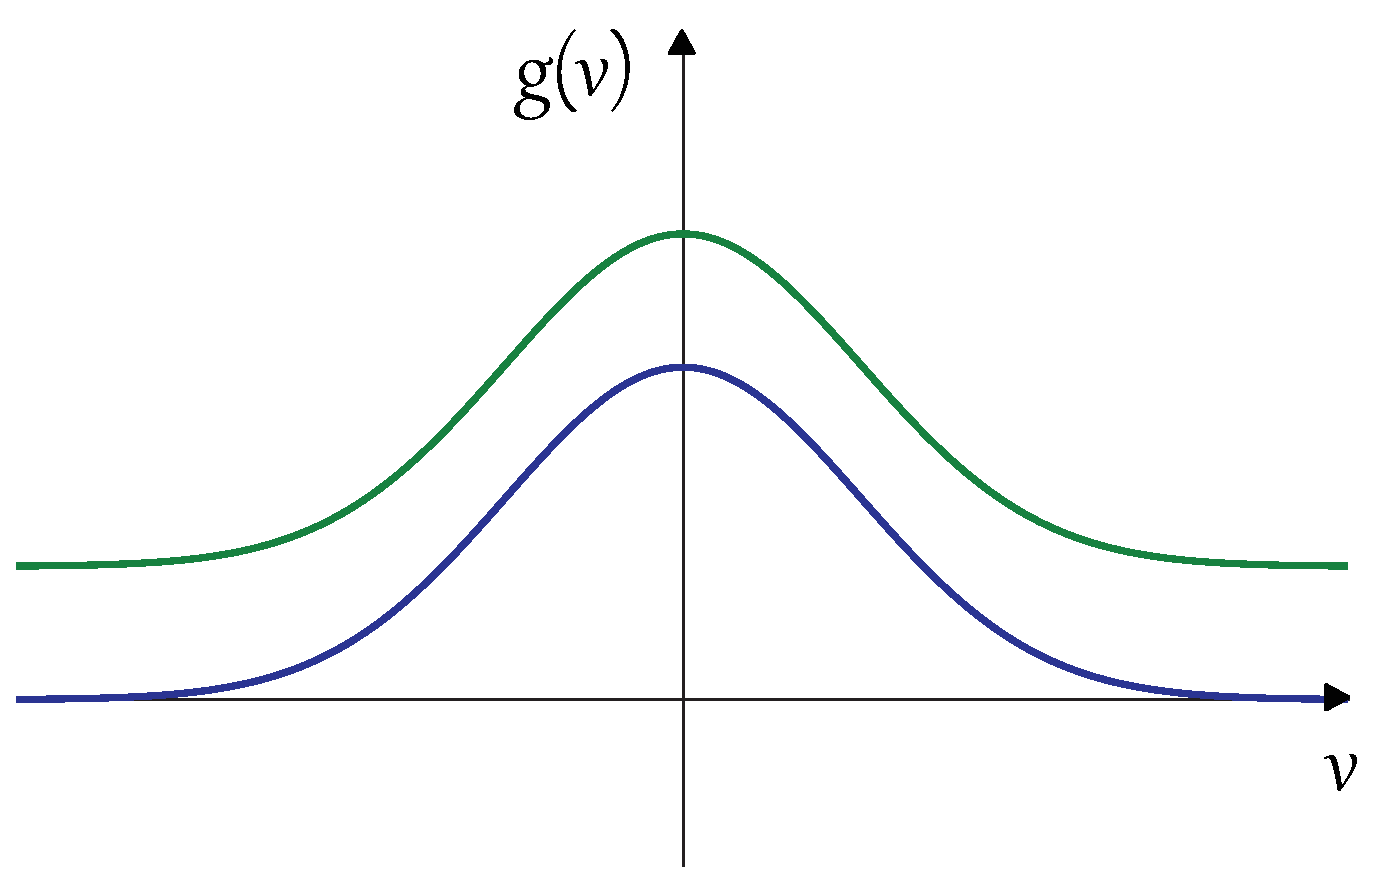
\includegraphics[width=0.45\textwidth]{images/g_gvc}
		\label{fig:g_gvc}
	}
	\subfigure[] {
		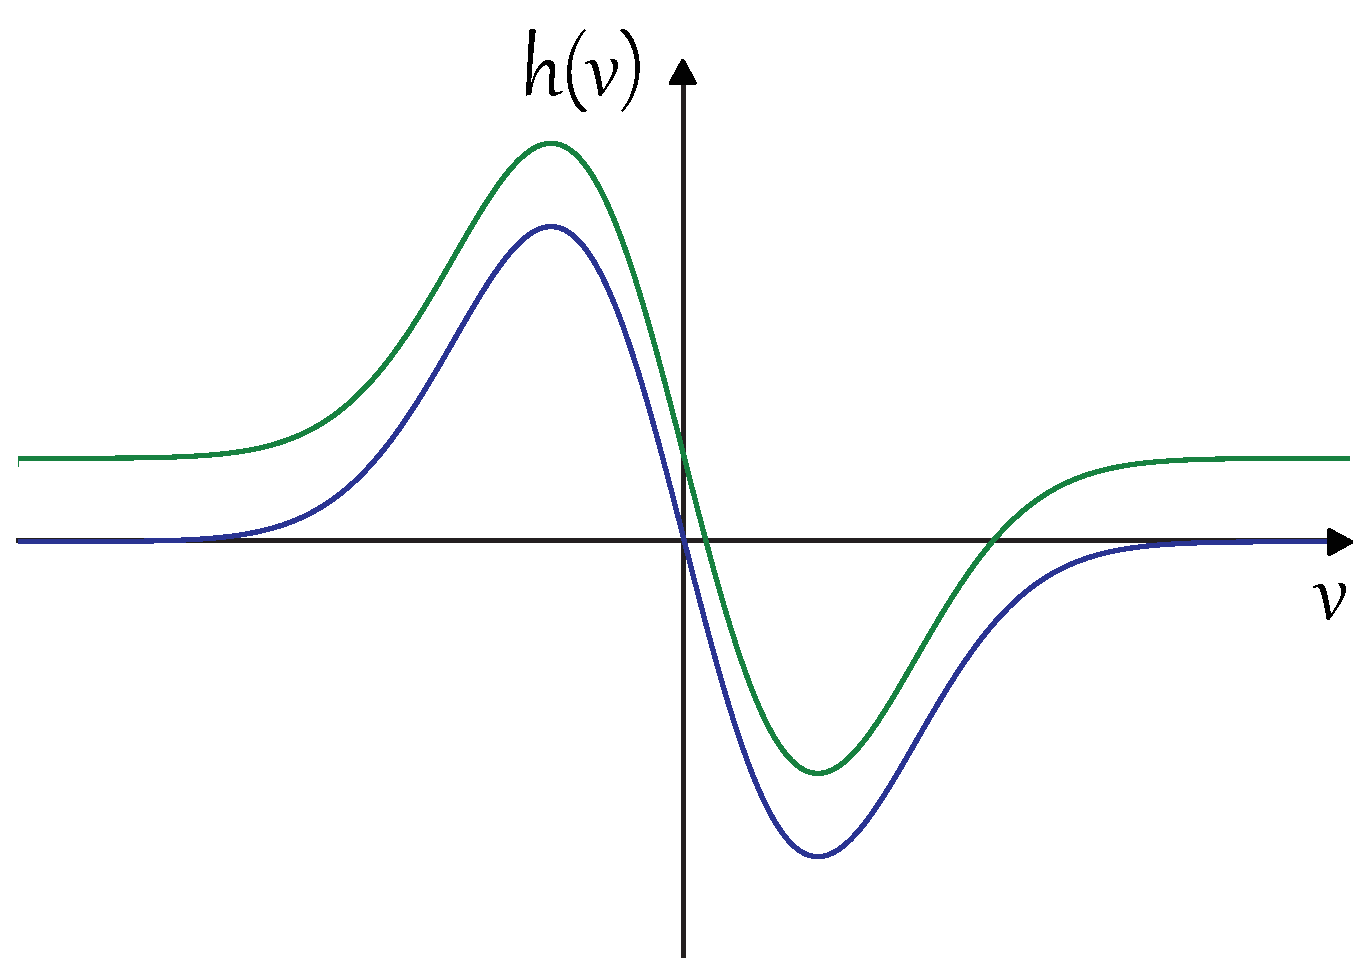
\includegraphics[width=0.45\textwidth]{images/g_hvc}
		\label{fig:g_hvc}
	}
	\caption{Deslocamento constante na imagem das funções $ g(v) $ e $ h(v) $.}
	\label{fig:g_shift}
\end{figure}

	No capítulo seguinte, uma nova metodologia é proposta para gerar funções de transferência 1D, utilizando o mesmo modelo de fronteira de \textit{Kindlmann e Durkin}~\cite{gordon}. As funções médias das derivadas de $ f(x) $ serão exploradas a fim de compor uma FT com mesmo peso, além de eliminar o $ g_{thresh} $.